\documentclass[a4paper,12pt]{article}
\usepackage{macros-ohp}


%Please make sure the tex is compiled twice to have all the background images displayed correctly.

\title{\Huge 
\textbf{ Study and Application of Concept-Extraction Algorithms in Statistical and Programming Sciences}
}

\author{
\Huge  Ana-Maria Vintila\\
	\Large Supervised by  Professor Brenda Vo \\
	\Large  University of New England, Australia\\
}
\date{}

% Ana
% My line spacing for the title page: 
\linespread{1.0}  % was 1.5

\begin{document}
	\begin{titlingpage}
	
	
	% Ana: set up animation settings -----------------
   %\animategraphics[autoplay,loop,height=5cm]{1}{imgs/rnn_step1_animation.png}{0}{47-1}
	
	% Ana: Making linespread on title page larger
	\linespread{1.5}
	\tikz[remember picture,overlay] \node[opacity=1,inner sep=0pt] at (current page.center){
\includegraphics[width=\paperwidth,height=\paperheight]{imgs/background.png}};
	\vspace*{3.5cm}
	{\let\newpage\relax\maketitle}
	\vspace*{\fill}
	\begin{textblock*}{140mm}(70mm,200mm)
			\begin{center}
				\begin{small}
		Vacation Research Scholarships are funded jointly by the Department of Education and Training
and the Australian Mathematical Sciences Institute.
				\end{small}
			\end{center}
	\end{textblock*}

	\end{titlingpage}

% ----------------------------------------------------------------
% Report Start


{\centering \section*{Abstract}} \label{sec:Abstract}

\vspace{-10pt}

{\small {\color{Red} (!) TODO: This is just some text here that i must later change in order to complete this presentation. This is some text that has overlap with the introduction, summarizes the project, and does not contain referencs. Oh, also remember it can be read independently of the entire report itself. }}


\section{Introduction: Motivation for Text Processing} \label{sec:Introduction} 

Vast amounts of knowledge are trapped in presentation media such as videos, html, pdfs, and paper as opposed to being concept-mapped, interlinked, addressable and reusable at fine grained levels. This defeats knowledge exchanges between humans and between human cognition and AI-based systems.

It is known that concept mapping enhances human cognition. Especially in domain-specific areas of knowledge, better interlinking would be achieved if concepts would be extracted using surrounding context, accounting for \hyperref[sec:Polysemy]{polysemy} and key phrases. ``You shall know a word by the company it keeps" (Firth, 1957). 

In my project I seek to understand models that create good language representations using lexical and semantic structure, at the \emph{\hyperref[nlptask:namedentityrecognitionNER]{entity} and \hyperref[nlptask:keyphraseextraction]{phrase} level}. 

Previous count-based models like \nameref{sec:Glove} and \nameref{sec:Word2Vec} motivated recent models like models like \nameref{sec:Transformer}, \nameref{sec:ELMo}, \nameref{sec:BERT}, \nameref{sec:TransformerXL}, \nameref{sec:XLNet}, and \nameref{sec:ERNIE_2} to move beyond simple co-occurrence counts to extract meaning. \nameref{sec:ERNIE_2} instead ``broadens the vision to include more lexical, syntactic and semantic information from training corpora in form of named entities (like person names, location names, and organization names), semantic closeness (proximity of sentences), sentence order or discourse relations" (Sun et al., 2019). For instance, \nameref{sec:ERNIE_1} can associate entire entity names with other terms in a given sentence, while on the same data, \nameref{sec:BERT} lacks this ability.

\emph{\textbf{Aims of this Research}}
\vspace{-7pt}
\begin{enumerate}
    \item "Study:" I will inventory, study, and compare architectures and frameworks to learn how they leverage entities,  \hyperref[sec:Polysemy]{polysemy} and contextual meaning for future study in concept extraction and natural language understanding.
    
    \item "Application:" using the PyTorch deep learning library, I aim to illustrate key model architecture while applying the model  to \nameref{nlptask:machinetranslationMT}.
\end{enumerate}
 
 
 
\textbf{Statement of Authorship: }

This report is planned and written entirely by me, and I cite authors of each model, where applicable. I learned from and adapted the PyTorch Code for the \nameref{nlptask:machinetranslationMT}task using GitHub. 

%\emph{\textbf{Layout of this Report}}

%\hyperref[sec:WordEmbeddings]{Section 1} of this report defines and examines usage of word embeddings in NLP; \hyperref[sec:LanguageModels]{Section 2} explains basic building blocks of the forthcoming models, and the latter sections discuss the different models: \nameref{sec:Word2Vec}, \nameref{sec:Glove}, \nameref{sec:Seq2Seq}, \nameref{sec:Transformer}, \nameref{sec:ELMo}, \nameref{sec:BERT}, \nameref{sec:TransformerXL}, \nameref{sec:XLNet}, and \nameref{sec:ERNIE}. 




\section{Word Embeddings}

Word embeddings, also called latent vector representations, which are fixed-length vector representations of words, have led to the success of many NLP systems in recent years, across tasks like named entity recognition (NER), part-of-speech tagging (POS), parsing, and semantic role labeling (SRL) (Luong et al. 2013, p. 1).

\subsection{Usage of Word Embeddings in Natural Language Processing}
An important idea in linguistics is that words used in similar ways have similar meanings (Firth, 1957). A distributional view of word meaning arises when accounting for the full distribution of contexts in a corpus where the word is found. For instance, words that tend to occur in the same neighboring context can be clustered to signify they have similar meaning. A key idea in NLP is suggests that information lives in text corpora and people and machines can use programs to collect and organize this information for use in NLP. With the onset of ever-larger text collections on the web, these programs have progressed from count-based statistics to more advanced methods. There are many insights into the power of word embeddings; similar words being close together allows generalization from one sentence to a class of similar sentences. For instance "the wall is blue" to "the ceiling is red" (Smith, 2019, p. 4). Put succinctly, "distributed representations words in a vector space help learning algorithms to achieve better performance in natural language processing tasks by grouping similar words" (Mikolov et al. 2013a, p. 1). 


\subsection{Intuitive Definition of Word Embeddings}
In the world of natural language processing, word embeddings are a collection of unsupervised learning methods for capturing semantic and syntactic information about individual words in a compact low-dimensional vector representation. Embedding methods analyze text data, learning distributed semantic representations of the vocabulary to capture its co-occurrence statistics. These learned representations are then useful for reasoning about word usage and meaning (Melamud et al. 2016, p. 1). 

Word vectors can be also calculated from sentences, phrases, or characters to create sentence embedding, phrase embedding, or character embedding, respectively. Character embeddings can be used to explain language morphology. For example, the following variants of the word "would" in social media would have similar character embeddings because they are spelled similarly: "would", "wud", "wld", "wuld", "wouldd", "woud", and so on (Smith, 2019, p. 5). 

Tokenization is the task-specific process of segmenting text into machine-understandable language. The term "tokens" describes words but also punctuation, hyperlinks, and possessive markers, such as apostrophes (Mohler, 2018). For example, lemma-based tokenization would specify that the tokens "cat" and plural "cats" would mean one word with the same stem or core meaning-bearing unit. Other forms of tokenization exist to differentiate word form, so those would be distinct tokens. Sentences and even characters can be tokenized out of a paragraph (Chromiak, 2017). 

\subsubsection{Analogical Reasoning Property of Word Embeddings}
Word embeddings can also represent analogies that have been encoded in the difference vectors between words. For example, gender differences can be represented by a constant difference vector, enabling mathematical operations between vectors based on vector space semantics (Colah, 2014). The famous analogy "man is to woman as king is to queen" can thus be expressed using learned word vectors as follows: $vector(man) - vector(woman) = vector(king) - vector(queen)$ (Smith, 2019). In the NLP task of machine translation, this property of learned word vectors would suggest the two languages being translated have a similar 'shape' and "that by forcing them to line up at different points, they overlap and and other points get pulled into the right positions" (Colah, 2014).

\subsection{Mathematical Overview For Word Embeddings}
 
A word embedding $W: [Words] \rightarrow R^n$ is a parametrized function mapping words in a language to an $n$-dimensional numeric vector. An example is: 

\begin{figure}[h]
\centering
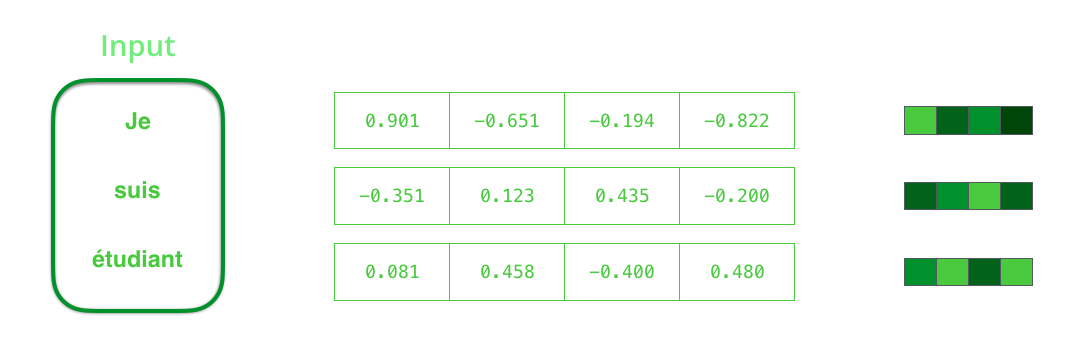
\includegraphics[width=0.8\textwidth]{example_word_embedding.png}
\caption{Example Word Embeddings. From \emph{Visualizing Neural Machine Translation Mechanics of Seq2Seq Models with Attention}, by Jay Alammar, 2018. \url{http://jalammar.github.io/visualizing-neural-machine-translation-mechanics-of-seq2seq-models-with-attention/}. Copyright 2018 by Jay Alammar.}
\end{figure}

According to Rudolph et al. (2016), "each term in a vocabulary is associated with two latent vectors, an \emph{embedding} and a \emph{context vector}. These two types of vectors govern conditional probabilities that relate each word to its surrounding context." 
Rudolph and Blei (2017) note that a word embedding uses vector representations to parameterize the conditional probabilities of words in a surrounding context. 
In other words, a word's conditional probability combines its \emph{embedding} and \emph{context vectors} of surrounding words, with different methods combining them differently. Subsequently, word embeddings are fitted to given text data by maximizing the conditional probabilities of observed text (Rudolph et al. 2017). 

\subsection{Static Embeddings vs. Contextual Embeddings}

\subsubsection{What is Polysemy?}

Polysemy means that a word can have multiple, distinct meanings. The distributional hypothesis in NLP states that meaning depends on context, and words occurring in the same contexts have similar meaning (Wiedemann et al. 2019). 

\subsubsection{The Problem With Static Embeddings: A Context-Free Representation}

Classic word vectors, also called static embeddings, represent words in a low-dimensional continuous space in a static way: this means each word has a single word vector representation regardless of its context (Ethayarajh, 2019). Skip-gram (Mikolov et al., 2013a) and GloVe (Pennington et al., 2014) are well-known algorithms for producing these "context-independent representations," as Peters et al. (2018) calls them, due to the fact that their word embedding matrix, inputted to a neural network representation, is trained to use co-occurring information in text, rather than using dynamic computation offered by language models (Batista, 2018). Although still able to capture latent syntactic and semantic meaning by training over large corpora, static embeddings by definition create a single vector representation per word, so all senses of a polysemous word are collapsed within a single representation (Ethayarajh, 2019). 

\subsubsection{A Better Solution: Contextual Embeddings To Capture Polysemy}

A contextual word embedding (CWE) is

Recent efforts to capture polysemy for word embeddings cast aside the idea of using a fixed word sense inventory. This allows contextual embeddings to "not only create one vector representation for each [word] type in the vocabulary" but to also create separate vectors for each token in a surrounding context. Indeed, experiments show that contextual embeddings can capture word senses successfully (Wiedemann et al., 2019). Wiedemann concludes that this allows for a more realistic model of natural language; contextual embeddings have proven their superiority over static embeddings for many NLP tasks such as text classification (Zampieri et al., 2019) and sequence tagging (Akbig et al., 2018). Although contextualization models such as BERT, ELMo, ERNIE 2.0, and Transformer differ widely, modeling "sentence or context-level semantics together with word-level semantics proved to be a powerful innovation" in the NLP world (Wiedemann et al., 2019). 



----------------


\subsection{Word Embedding Representations: Count-Based vs. Context-Based}

LILIAN WENG: https://hyp.is/dKRaygVnEeqRaI-_7zzFtQ/lilianweng.github.io/lil-log/2017/10/15/learning-word-embedding.html
"There are two main approaches for learning word embedding, both relying on the contextual knowledge.

Count-based: The first one is unsupervised, based on matrix factorization of a global word co-occurrence matrix. Raw co-occurrence counts do not work well, so we want to do smart things on top.
Context-based: The second approach is supervised. Given a local context, we want to design a model to predict the target words and in the meantime, this model learns the efficient word embedding representation."


One way to convert human text into machine-interpretable data is to use a one-hot encoding. Essentially, each distinct word stands for one dimension of the resulting vector a




\subsection{How Word Embeddings are Used}

To complete NLP tasks, NLP models usually choose to use probability as a measure to evaluate a language model. 

Word embeddings are trained as parameters to optimize a generic task-independent objective function. 

Word embeddings are generally fed as vector parameters into a neural network language model. Each row of a word embedding matrix corresponds to a word in the vocabulary, which consists of unique tokens from a corpus. 

The word embedding matrix corresponds to the weights of the neural network, which are trained to minimize an objective or loss function by backpropagating gradients over the neural network. 

Alternatively, we can view this loss function as maximizing the conditional probabilities of words. The conditional probability of a word combines its embedding and the context vectors of its surrounding words. Different language models combine them differently. 

In this way, distributional semantics arises as word embeddings learn to represent context via proximity of related words.  

\section{Language Models} \label{sec:LanguageModels}

A language model takes a sequence of word vectors and outputs a sequence of predicted word vectors by learning a probability distribution over words in a vocabulary. In representation terms, the ``vector representation of a word depends on the context vector representation" (Ibrahim, 2019).

Many tasks such as \nameref{nlptask:machinetranslationMT}, spell correction, text summarization, \nameref{nlptask:questionansweringQA}, and \nameref{nlptask:sentimentanalysisSA} all use language models to convert text into machine-interpretable language (Chromiak, 2017). 

Intuitively, language models predict words in a blank. For instance, given the following context: ``The $\_\_\_$ sat on the mat" where $\_\_\_$ is the word to predict, a language model might suggest the word ``cat" should fill the blank a certain percentage of the time and the word ``dog" would fill the blank with lower probability (Kurita, 2019). 

Formally, language models work by computing the conditional probability of a word $w_t$ given a context, such as its previous $n-1$ words, where the probability is: $P(w_t | w_{t-1}, ..., w_{t-n+1})$ (Ruder, 2016). Chromiak adds that the probability chain rule is the main tool used to find the joint probability of a word sequence. For events A and B, the probability chain rule states:
$$
P(A | B) = \frac{P(A \cap B)} {P(B)}
$$
which lends the following formula for a set of $T$ word tokens $w_1, ..., w_T$ from a sentence $S$: 
$$
\begin{array}{ll}
P(S)
&= P \Big(w_1, ..., w_T \Big)  \\
&= P(w_1) \cdot P(w_2 \; | \; w_1) \cdot ... \cdot P(w_n \; | \; w_1, ..., w_{T-1}) \\
&= \prod_{t=1}^T P \Big(w_t \; | \; w_1, ..., w_{t-1} \Big) \\
\end{array}
$$
Typically, the \textbf{Markov Assumption}, which states that the probability of a word depends only on its previous word, is used to reduce context history and thus intake of model data. Thus the joint probability is estimated using the $n$ previous words of the current word $w_t$:
$$
P \Big(w_1, ..., w_T \Big) \approx \prod_{t=1}^T P \Big(w_t \; | \; w_{t-1}, ..., w_{t-n+1} \Big)
$$

There are several kinds of language models. 

\subsection{N-gram Language Model} \label{sec:NGramLM}

An $n$-gram is a sequence of $n$ words. The $n$-gram language model is one of the simplest models that assigns probabilities to sentences and word sequences. It calculates a word's probability based on the frequencies of its constituent $n$-grams, taking just the preceding $n-1$ words as context instead of the entire corpus (Ruder, 2016): 
$$
P \Big(w_t \; | \; w_{t-1}, ..., w_{t-n+1} \Big) = \frac {count(w_{t-n+1},...,w_{t-1},w_t)} {count(w_{t-n+1},...,w_{t-1})}
$$

\subsection{Neural Network Language Model} \label{sec:NeuralLM}

\subsubsection{Curse of Dimensionality} \label{sec:CurseDim}

Bengio et al. (2003) defines the \emph{curse of dimensionality} in NLP as how a word sequence may differ from the training set of word sequences. This appears when modeling the joint distribution between discrete random variables (like words in a sentence). 

\subsubsection{Key Concept: Neural Network Representation} \label{sec:NeuralNetRepr}

A \textbf{neural network} is a function from vectors to vectors.  

All neural network representations rely on a structure called a neuron, which is expressed as a linear formula: $W \cdot x + b$. By applying a nonlinear function $f(\cdot)$ to this equation and by incorporating many hidden layers and by stacking neurons together, a neural network can model any function. A neuron is shown in \cref{fig:neuron}.

\begin{figure}[h]
\vspace{-5pt}
\centering
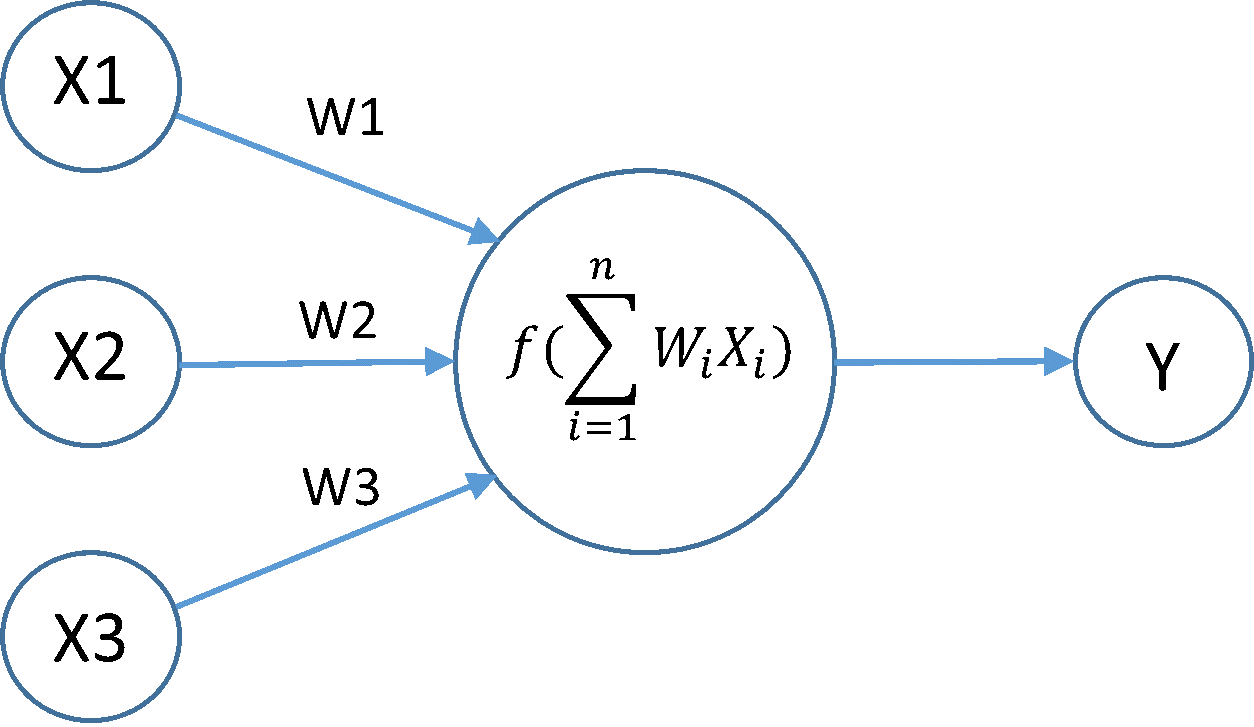
\includegraphics[width=0.35\textwidth]{neuron.png}
\vspace{-5pt}
\caption{\footnotesize Neuron. From \emph{Applying Unsupervised Machine Learning to Sequence Labeling}, by Jacob, 2019. \url{https://medium.com/mosaix/deep-text-representation-for-sequence-labeling-2f2e605ed9d}. Copyright n.d. by n.d.}
\vspace{-5pt}
\label{fig:neuron}
\end{figure}

Many \hyperref[app:Appendix_NLPTasks]{NLP applications} using neural networks feed in word tokens that is transformed based on its context words, resulting in an updated version of the word embedding (Smith, 2019). Embeddings are fed as parameters or weights into a neural network which \emph{optimizes} them to best fit the text by minimizing a continuous loss function using gradient-descent based algorithms. Every neural network representation consists of three components (Ruder, 2016):

\begin{enumerate}
    \item \textbf{Embedding Layer}\label{cnc:embeddingLayer}: this layer creates word embeddings by multiplying an index vector with a word vector matrix. 
    
    \item \textbf{Intermediate Layer(s)}: multiple layers are used to create a fully-connected layer that applies a non-linearity function (like hyperbolic tangent or sigmoid) to the concatenation of word embeddings. 
    
    \item \textbf{Softmax Layer}\label{cnc:softmaxLayer}: the last layer normalizes the word embedding matrix to using a \textbf{softmax function} to create a probability distribution over words $w_t$ in the vocabulary. 
    $$
    P \Big(w_t \; | \; w_{t-1}, ..., w_{t-n+1} \Big) = \frac {\exp{ \Big(h^T \cdot v_{w_t}' \Big) }} {\sum_{w_i \in V} \exp{ \Big(h^T \cdot v_{w_i}' \Big) }}
    $$
    where $V = $ vocabulary of a corpus, $h = $ output vector of the hidden layer, and $v_w' = $ the output embedding of word $w$. 
\end{enumerate}

Many neural networks are \textbf{feed-forward neural network (FNN)}\label{cnc:ffn}s, in which input is fed in the forward direction only. 


\subsubsection{Solution to Curse of Dimensionality: Neural Model and Continuous Vector Representations} \label{sec:SolutionToCurseDim}

The $n$-gram model seeks to remedy the \emph{curse of dimensionality} by combining short overlapping word sequences seen in the training set. 

However, Bengio et al. (2003) developed a \emph{neural probabilistic language model} to learn a \hyperref[sec:DistributedRepr]{distributed representation} for words to allow the model to generalize to unseen data. The neural model does two tasks simultaneously; (1) it learns a \hyperref[sec:DistributedRepr]{distributed representation} for each word, and also (2) it learns the probability distribution of word sequences \emph{as a function of} the \hyperref[sec:DistributedRepr]{distributed representations}. The model generalizes to unseen data successfully because unseen word sequences get a high probability if containing words that are similar to words that were already seen.  

Advantageously, this model can capture longer contexts better than the \hyperref[sec:NGramLM]{$n$-gram}, which is limited to short contexts. As a result of continuous word vector representations, the learned probability function's parameters increase linearly not exponentially with the vocabulary size, and they increase linearly with vector dimension, thus resolving the curse of dimensionality (Bengio et al., 2003).  

For more information, \nameref{app:Appendix_Backprop} mathematically explains how neural networks learn parameters. 


\subsection{Bidirectional Language Model} \label{sec:BidirectionalLM}

\subsubsection{Forward Language Model} \label{sec:ForwardLM}

A general language model predicts a next word given its context words, $P(\textit{Word} \: | \: \textit{Context})$. 

A \textbf{forward language model} takes this context to be previous words. From Peters et al. (2018), given a sequence of $N$ tokens $(t_1, t_2, ..., t_N)$, a forward language model calculates the probability of the tokenized sentence assuming the probability of a word token $t_k$ is conditional on its history tokens, $(t_1, ..., t_{k-1})$:
$$
P \Big(t_1, t_2, ..., t_N \Big) = \prod_{k=1}^N P \Big(t_k \; | \; t_1, t_2, ..., t_{k-1} \Big)
$$

\subsubsection{Backward Language Model} \label{sec:BackwardLM}

A \textbf{backward language model} is similar to a forward model excepts it predicts the current token $t_k$ conditional on future context tokens:
$$
P \Big(t_1, t_2, ..., t_N \Big) = \prod_{k=1}^N P \Big(t_k \; | \; t_{k+1}, t_{k+2}, ..., t_N \Big)
$$

\subsubsection{Combining Forward and Backward}

A \textbf{bidirectional language model (biLM)} such as in \cref{fig:bidirectionalLM} combines the \hyperref[sec:ForwardLM]{forward} and \hyperref[sec:BackwardLM]{backward language model}s and uses maximum likelihood estimation to \emph{jointly} maximize the log likelihood of the forward and backward directions: 
$$
\sum_{k=1}^N \Big( \text{log} \Big( P \Big(t_k \; | \; t_1,...,t_{k-1}; \; \overrightarrow{\theta} \Big) + \text{log} \Big( P \Big(t_k \; | \; t_{k+1}, t_{k+2}, ..., t_N; \; \overrightarrow{\theta} \Big) \Big)
$$
where $\overrightarrow{\theta}$ represents additional parameters (Peters et al., 2018). 


\begin{figure}[h]
\vspace{-5pt}
\centering
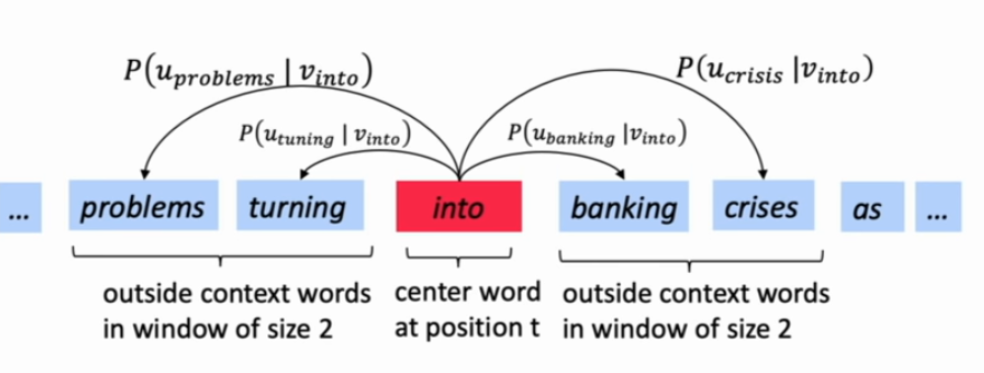
\includegraphics[width=0.6\textwidth]{bidirectional_languagemodel_banking.png}
\vspace{-5pt}
\caption{\footnotesize Example Bidirectional Language Model. From \emph{Word2Vec Overview With Vectors}, by CS224n: Natural Language Processing with Deep Learning (Stanford), 2018. \url{https://sangminwoo.github.io/2019-08-28-cs224n-lec1/}. Copyright n.d. by n.d.}
\vspace{-5pt}
\label{fig:bidirectionalLM}
\end{figure}

Akbik et al. (2018) use the hidden states of a bidirectional recurrent neural network to create contextualized word representations. 

For example, consider the sentences ``Mary accessed the bank account" and ``The swan waded to the bank of the river." In the first sentence, a unidirectional contextual model would represent the target word ``bank" based on `I accessed the' but not `account,' thus failing to capture the polysemy of `bank.' But a bidirectional language model represents ``bank" using both previous and next context to ameliorate this problem.

\section{Word2Vec Model}

\subsection{Word Embedding Representations: Count-Based vs. Context-Based}
 
Word embeddings can be learned using two kinds of contextual vector space models: the \textbf{count-based} or \textbf{context-based vector space models}. 

\textbf{Count-based vector space models} are unsupervised learning algorithms based on matrix factorization of a global word co-occurrence matrix. The main assumption is words in similar contexts share related semantic meanings. Examples include PCA and neural probabilistic language models. Another term for this type is \textbf{distributed semantic model} (DSM) (Weng, 2017). 

\textbf{Context-based vector space models} are supervised algorithms that use a local context to predict target words. These are predictive models which take dense word vectors as parameters and update word representations during training.

In 2014, Baroni et al. showed that predictive approaches outperformed count models significantly and consistently. 

Although \textbf{Word2Vec} and \textbf{GloVe} are predictive and context-based vector space models, they still rely on co-occurrence counts. 

\textbf{Word2Vec} is an unsupervised learning algorithm for obtaining word vector representations using a two-layer neural network. Its input is the text corpus and output is the set of feature vectors, as one vector per word. Existing word representations already capture linguistic patterns, allowing algebraic operations to be done on the word vectors in their semantic vector space; for example, $vector(\textit{"King"}) - vector(\textit{"Man"}) + vector(\textit{"Woman"})$ outputs a vector close to the word vector for ``Queen". But Mikolov et al. (2013b) created the \textbf{Skip-Gram} and \textbf{CBOW} as part of \textbf{Word2Vec} to learn word vector representations more efficiently from large data. Previous architectures used fewer words and smaller vector dimensionality, thus reducing the quality of the learned representations. 

\subsubsection{One-Hot Encodings}

A key concept for what follows is \textbf{one-hot vector encoding}. This is the simplest type of word embedding where each cell in the vector corresponds to a distinct vocabulary word, thus its dimension equals the vocabulary size. A $1$ is placed in the cell marking the position of the word in the vocabulary, and a $0$ is placed in all other cells. However, this can result in high-dimensionality vector representations for large vocabularies, causing increased computational costs, and similarity between categories cannot be represented. 

\subsection{Basic Structure of Skip-Gram and CBOW}

Both the Skip-Gram and CBOW are neural network language models with one hidden layer. 

The input vector $\overrightarrow{x} = (x_1,..., x_V)$ and output vector $\overrightarrow{y} = (y_1,...,y_V)$ are both \textbf{one-hot encodings}, and the hidden layer of the neural network is a word embedding with dimension $N$. (Thus even though the vocabulary size is $V$, the goal is to learn embeddings with size $N$). For a specific time step $t$, the model predicts one output word $w_{t+j}$ whose vector representation is $\overrightarrow{y}$, given one input word $w_t$, whose vector representation is $\overrightarrow{x}$. 

For Skip-Gram, $w_{t+j}$ is the predicted context word while CBOW considers this he predicted target word. Also, $w_t$ is the input target word for Skip-Gram while the CBOW considers this the input context word. 

The vectors $v_w$ and $v'_w$ are two representations of word $w$; vector $v_w$ comes from the rows of the input layer $\rightarrow$ hidden layer weight matrix $W$, and vector $v'_w$ comes from the rows of the hidden layer $\rightarrow$ output layer weight matrix $W'$. We call $v_w$ the \textbf{input vector} and $v'_w$ is the \textbf{output vector} of the word $w$. 


\subsubsection{Skip-Gram Model}

The Skip-Gram model predicts context words given a single target word. It uses a fixed sliding window $c$, or size of the training context, to capture context along a sentence. A target word thus has left and right context words within that sliding window. This target center word is represented as a \textbf{one-hot encoding} that is input to a neural network which updates the vector with values near $1$ in cells corresponding to predicted context words (Weng, 2017).

Consider the following sentence from Weng (2017): ``The man who passes the sentence should swing the sword." Using a context window size of $c = 5$ and target word ``swing", the Skip-Gram should learn to predict the context words $\{\texttt{"sentence"}, \texttt{"should"}, \texttt{"the"}, \texttt{"sword"} \}$, and so the target-context word pairs fed into the model for training are: (\texttt{"swing"}, \texttt{"sentence"}), (\texttt{"swing"}, \texttt{"should"}), (\texttt{"swing"}, \texttt{"the"}), and (\texttt{"swing"}, \texttt{"sword"}). 

The Skip-Gram is illustrated below. 

\begin{figure}[h]
\vspace{-5pt}
\centering
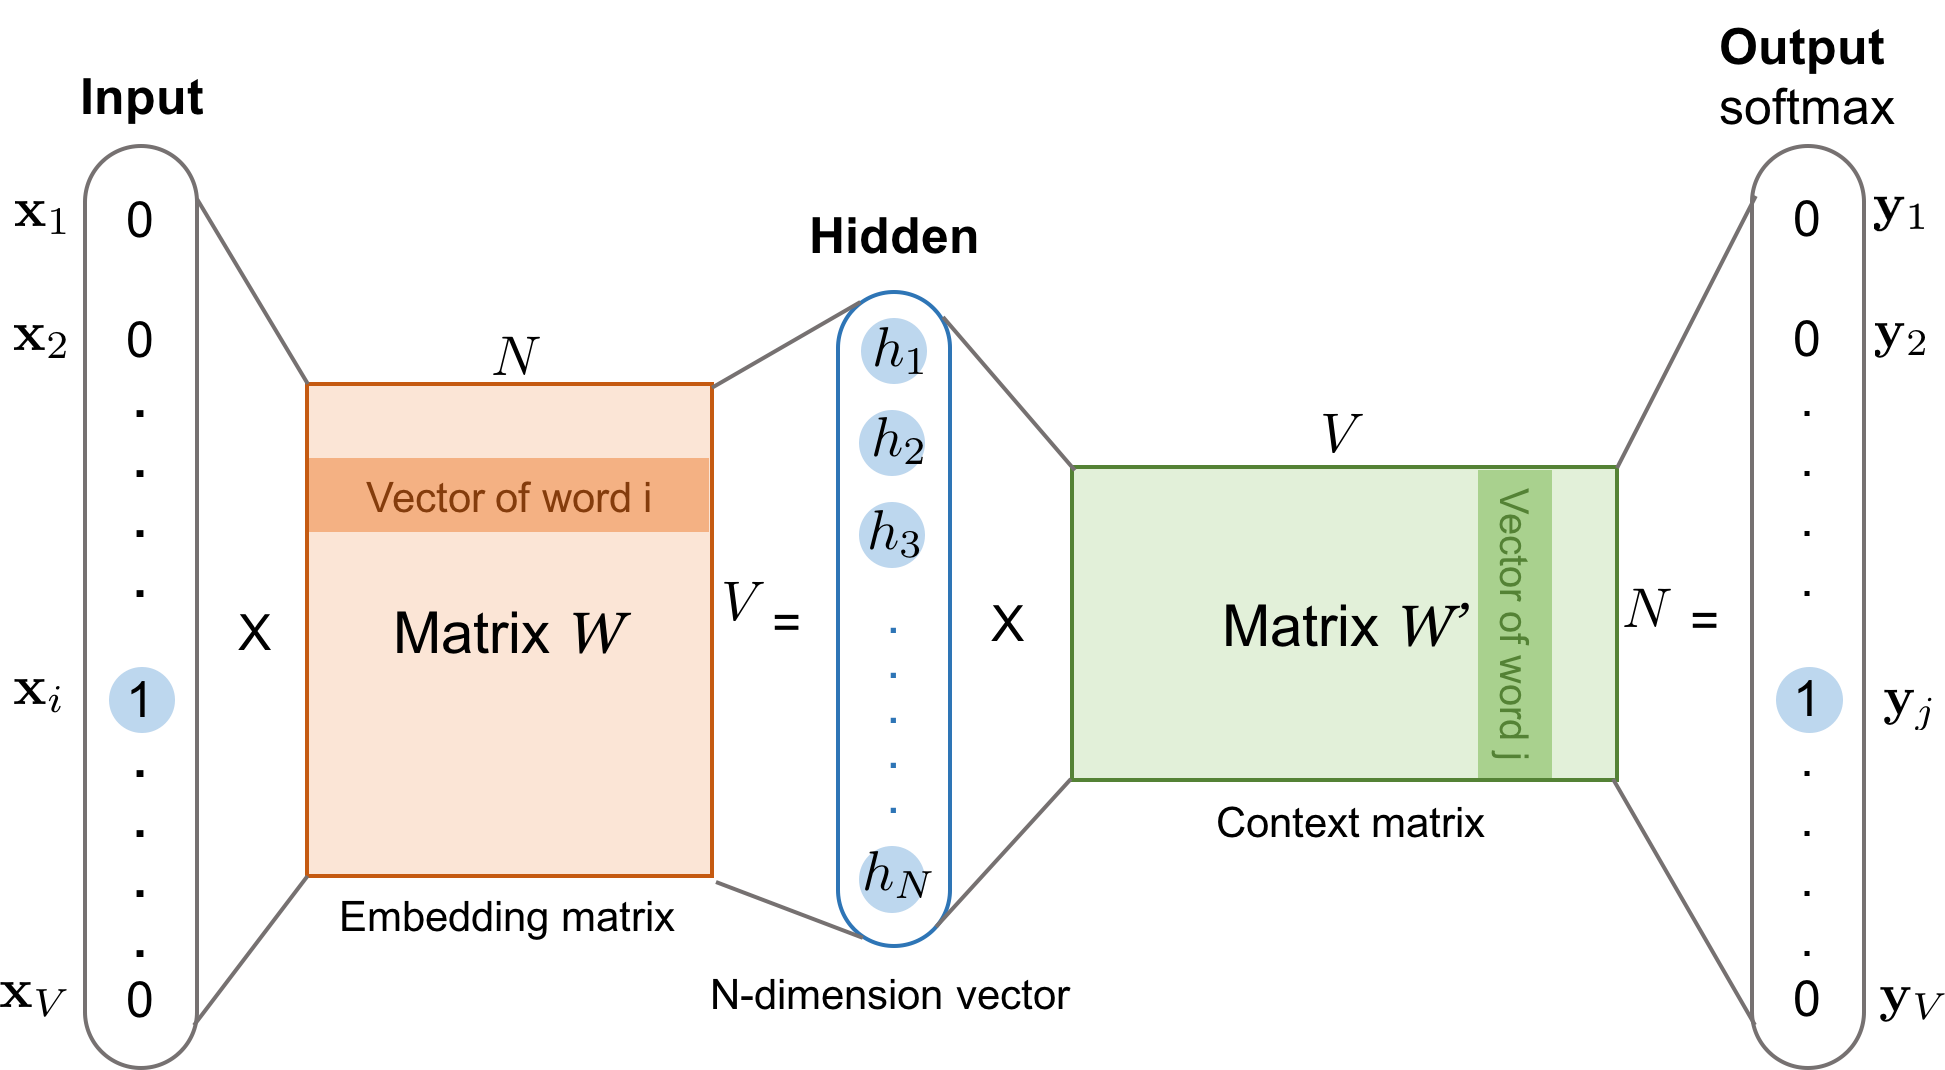
\includegraphics[width=0.6\textwidth]{imgs/skipgram_image.png}
\vspace{-5pt}
\caption{\footnotesize Skip-Gram Model; simplified version, with one input target word and one output context word. From \emph{Learning Word Embeddings}, by Lilian Weng, 2017. \url{https://lilianweng.github.io/lil-log/2017/10/15/learning-word-embedding.html}. Copyright n.d. by n.d.}
\vspace{-5pt}
\end{figure}

\subsubsection{Forward and Backward Pass for Skip-Gram}

According to Figure 4 above, the procedure for learning word vectors is: 

1. the input word $w_i$ and output word $w_j$ are encoded as one-hot vectors, $\overrightarrow{x}$ and $\overrightarrow{y}$ respectively. (For Skip-Gram, $\overrightarrow{x}$ is the target vector and $\overrightarrow{y}$ is the context vector). 

2. A randomly initialized word embedding matrix $W$ with size $V \times N$ at the input $\rightarrow$ hidden layer is multiplied with $\overrightarrow{x}$ to give the $N$-dimensional embedding for target word $w_i$. This embedding resides in the $i$-th row of $W$ and is considered as the hidden layer of the model. 

3. Next, the hidden layer is multiplied by weight matrix $W'$ with size $N \times V$ to produce the one-hot encoded output vector, $\overrightarrow{y}$. \textbf{NOTE: }the output context matrix $W'$ encodes words as context and is distinct from the embedding matrix $W$. 

4. The result of the above multiplication is sent through the softmax layer to create a probability distribution over the words. 

5. Errors are obtained by subtracting the output vector with the target vector. 

6. The error vector is backward-propagated through the neural network to update the weight matrix. The procedure continues until errors are small enough. 

\subsubsection{Loss Function for Skip-Gram}

The loss function is a key step for backward propagating errors through the neural network. Mikolov et al. (2013a) defines the loss function to be able to find word representations to predict the output word $w_{t+j}$ given an input word $w_t$. Formally, given the training word sequence $w_1, w_2, ..., w_T$ with $T$ training samples, the Skip-Gram maximizes the average log probability
$$
J_\theta = \frac{1}{T} \sum_{t=1}^T \sum_{-c \leq j \leq c, j \neq 0} \text{log} \Big(P \Big(w_{t+j} \;| \; w_t \Big) \Big)
$$
where $c$ is the training size context window. 

From Peters et al. (2013), the above probability in the loss function is:
$$
P \Big( w_{t+j} \; | \; w_t \Big) = \frac {\exp{ \Big( (v'_{w_{t+j}})^T  v_{w_t} \Big) }} {\sum_{w=1}^V \exp{ \Big( (v'_w)^T \cdot v_{w_t} \Big) }}
$$
where $w_t$ is the inputted target word, $w_{t+j}$ is the predicted context word, and $V$ is the number of vocabulary words. 



\subsubsection{Continuous Bag of Words Model (CBOW)}

The continuous bag of words model (CBOW) is opposite of the Skip-Gram since it predicts the \emph{target} word based on a \emph{context} word. In the general case, CBOW receives a window of $n$ context words around the target word $w_t$ at each time step $t$ and tries to predict the target word. The CBOW is called ``continuous" bag-of-words since it uses continuous distributed representations of the context words whose order is not important (Mikolov et al., 2013b). 

The CBOW is illustrated below: 

\begin{figure}[h]
\vspace{-5pt}
\centering
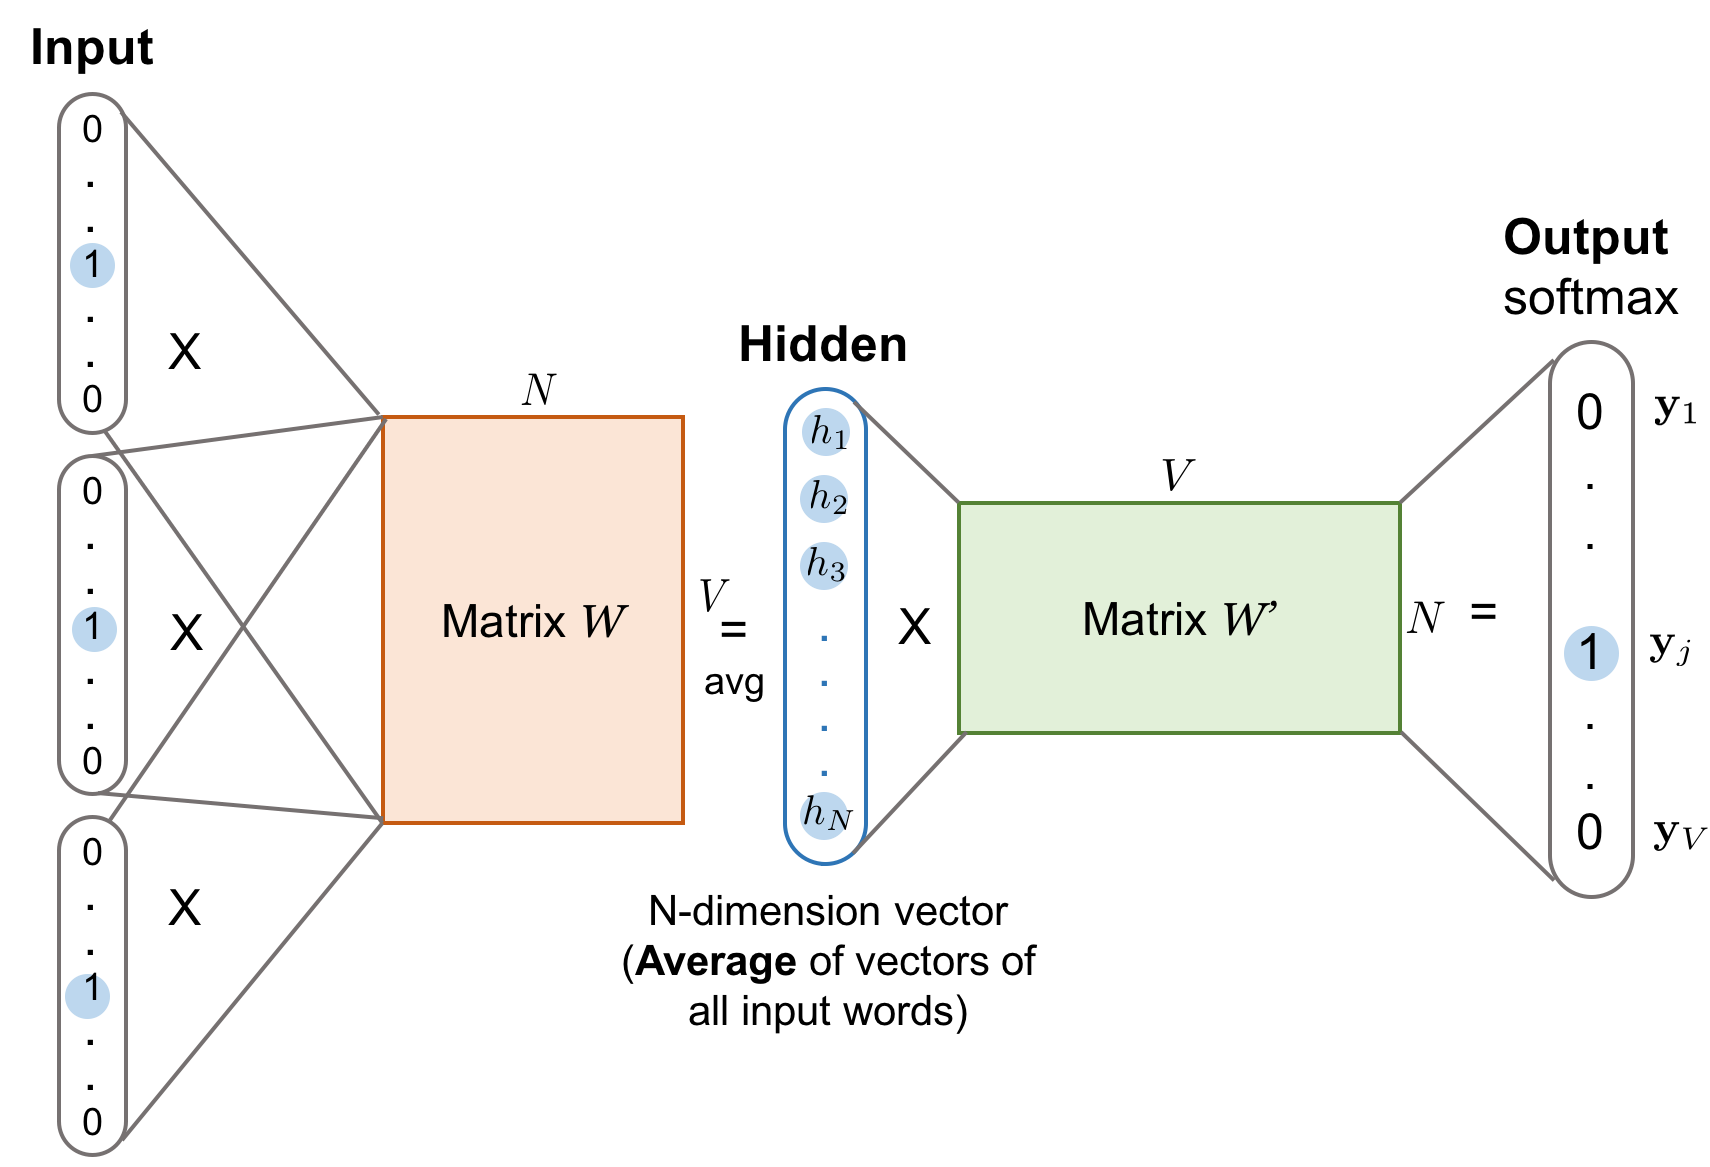
\includegraphics[width=0.6\textwidth]{imgs/cbow.png}
\vspace{-5pt}
\caption{\footnotesize CBOW Model with several one-hot encoded context words at the input layer and one target word at the output layer. From \emph{Learning Word Embeddings}, by Lilian Weng, 2017. \url{https://lilianweng.github.io/lil-log/2017/10/15/learning-word-embedding.html}. Copyright n.d. by n.d.}
\vspace{-5pt}
\end{figure}

\subsubsection{Forward and Backward Pass for CBOW}

The forward pass for CBOW is similar to Skip-Gram's. The key difference is due to having multiple context words: the CBOW averages the context word vectors while multiplying the input vector $\overrightarrow{x}$ and input $\rightarrow$ hidden layer matrix $W$. Rong (2016) describes the hidden layer calculation as: 
$$
\begin{array}{ll}
\overrightarrow{h} 
&= \frac{1}{c} W \cdot \Big(\overrightarrow{x_1} + \overrightarrow{x_2} + ... + \overrightarrow{x_c} \Big) \\
&= \frac{1}{c} \cdot \Big(\overrightarrow{v_{w_1}} + \overrightarrow{v_{w_2}} + ... + \overrightarrow{v_{w_c}} \Big)
\end{array}
$$
where $c$ is the number of context words, $w_1,...,w_c$ are the context words, and $v_w$ is the input vector for general word $w$. 

According to Weng (2016), the fact that CBOW averages distributional information of the context vectors makes it better suited for small datasets. 

\subsubsection{Loss Function for CBOW}

On the output layer, the CBOW outputs $c$ multinomial distributions, for each of the $c$ context words. The training object is to maximize the conditional probability of observing the true output word given several context words, while accounting for their weights. 

From Ruder (2016), the loss function is: 
$$
J_\theta = \frac{1}{T} \sum_{t=1}^T \text{log} \Big( P \Big( w_t \; | \; w_{t-n}, ..., w_{t-1}, w_{t+1}, ..., w_{t+n} \Big) \Big)
$$
where $n$ is number of context words and $w_{t-n}, ..., w_{t+n}$ are context words around the target word $w_t$. 

From Rong (2016), the above probability in the loss function, for the one context word case, is:
$$
P \Big( w_t \; | \; w_I \Big) = \frac {\exp{ \Big( (v'_{w_O})^T  v_{w_I} \Big) }} {\sum_{w=1}^V \exp{ \Big( (v'_w)^T \cdot v_{w_I} \Big) }}
$$
where $w_I$ is the input context word, $w_O$ is the predicted target word, and $V$ is the number of vocabulary words. 


\subsection{Phrase-Learning Attempt in Word2Vec Using Skip-Gram}

Mikolov et al. (2013a) state that a problem with previous word vectors is their lack of phrase representation - the phrases ``Canada" and ``Air" could not be recognized as part of a larger concept and thus combined into ``Air Canada". Many phrases have meaning that is not just a composition of the meanings of its individual words and should be represented as their own unique tokens in the training data. In contrast, a bigram like ``this is" should remain unchanged (Mikolov et al., 2013a, p. 5). 

To solve this issue, the Skip-Gram was updated using a data-driven scoring technique. Phrases are formed based on unigram and bigram counts: 
$$
S_{phrase} = \frac{C(w_i w_j) - \delta} {C(w_i)C(w_j)}
$$
where $C(\cdot)$ is the count of a unigram $w_i$ or bigram $w_i w_j$ and $\delta$ is a discounting threshold to avoid formation of infrequent words and phrases. High values of $S_{phrase}$ means the phrase is most likely a phrase rather the simple concatenation of two words. 

Regarding model accuracy, Mikolov et al. (2013a) found that the phrase Skip-Gram model with hierarchical softmax and subsampling performed significantly better on a large data set than the original Skip-Gram without the phrase feature. 

It was found that the phrase Skip-Gram exhibits a linear structure \textbf{additive compositionality} of word vectors, which allows words to be combined meaningfully by adding their word vectors. For instance, composing word vectors $vector(\texttt{"French"}) + vector(\texttt{"actress"})$ results in the phrase $vector(\texttt{"Juliette Binoche"})$. 

This \textbf{additive compositionality} feature of word vectors stems from the loss function's formulation. Since learned context vectors can represent the overall distribution of context words in which the target word appears, and since the vectors are logarithmically related to the probabilities from the output layer, the sum of two word vectors is related to the product of the context distributions (using the logarithm sum rule). This product of distributions functions like an AND function since words are weighted by probability. Consequently, if the key phrase ``Volga River" appears many times in the same sentence along with ``Russian" and ``river", the sum $vector(\texttt{"Russian"}) + vector(\texttt{"river"})$ results in the phrase $vector(\texttt{"Volga River"})$ or at least a vector close to it (Mikolov et al., 2013a). 

\section{GloVe Model}

The Global Vectors for Word Representation (GloVe) model is an unsupervised learning algorithm that aims to capture meaning in a semantic vector space using global count statistics instead of only local contextual information (Pennington et al., 2014). The GloVe authors show that it is the \emph{ratio} of co-occurrence probabilities of two words rather than their actual probabilities that contains meaning and they carve out this information as vector offsets. 

\subsection{Problem with Word2Vec: Secret in the Loss Function}

A major deficiency in Word2Vec is that it only accounts for local contexts and ignores global count information. Kurita (2018) exemplifies that the words ``the" and ``cat" might be used together frequently but Word2Vec doesn't know if this is because ``the" is a common word or because ``the" and ``cat" are actually correlated. 

Pennington et al. (2014) say that Word2Vec implicitly optimizes over a co-occurrence matrix while streaming over input sentences. The key point is that Word2Vec optimizes the log likelihood of seeing words in the same context windows together, resulting in the below alternative way of expressing Word2Vec's loss function: 
$$
J = - \sum_i X_i \sum_j P_{ij} \text{log}(Q_{ij}) 
$$
where $X_i = \sum_k X_{ik}$ is the total number of words appearing in the context of word $i$ and $Q_{ij}$ is the probability that word $j$ appears in context of word $i$ and is estimated as a softmax: $Q_{ij} = \text{softmax} \Big( w_i \cdot w_j \Big)$. This shows that the loss of Word2Vec is just another form for cross entropy between the predicted and actual word distributions found in the context of word $i$. However the authors of GloVe say that cross entropy models long-tailed distributions poorly. Additionally, the cross-entropy here is weighted with factor $X_i$ which results from streaming over all data equally; so a word appearing $n$ times contributes to the loss $n$ times. 
However, there is no inherent justification for streaming across all words equally. In fact, GloVe computes differences between unnormalized probabilities, contrary to Word2Vec (Kurita, 2018). 


\subsection{Motivation for GloVe}

Previous models using global counts, such as Latent Semantic Analysis (LSA) produced word embeddings that lacked the interesting vector analogical property of word vectors produced by Word2Vec. Thus, they failed to capture ``dimensions of meaning" such as gender, grammar tense, and plurality, disabling downstream models from easily extracting meaning from those word vectors (Kurita, 2018). 

Building from past failures while avoiding Word2Vec's local context problems, GloVe instead uses a principled and explicit approach for learning these ``dimensions of meaning."


\subsection{Describing GloVe}

\subsubsection{Notation in GloVe}

Let $X$ be the matrix of word co-occurrence counts; let $X_{ij}$ be the $ij$-th entry $X$ that counts how many times any word appears in the context of word $i$, and let $P_{ij} = p_{\text{co}} \Big(w_j \; | \; w_i \Big) = \frac {X_{ij}} {X_i}$ be the probability that word $j$ appears in the context of word $i$ (Pennington et al., 2014; Weng, 2017).

\subsubsection{Meaning Extraction Using Co-Occurrence Counts}

GloVe uses a co-occurrence matrix that describes how words co-occur within a fixed sliding window, relying on the assumption that counts and co-occurrences can reveal word meaning. Words are said to \textbf{co-occur} when they appear together within this fixed window (Kurita, 2018). Then, GloVe takes this matrix as input, rather than the entire corpus. Thus, sentence boundaries no longer matter since GloVe accounts for corpus-wide co-occurrence, rather than relying on co-occurrences from a sentence-level.

From Weng (2017), the co-occurrence probability is defined as: 
$$
P_{ik} = p_{\text{co}} \Big(w_k \; | \; w_i \Big) = \frac{C(w_i, w_k)}{C(w_i)}
$$
where $C(w_i, w_k)$ counts the co-occurrence between words $w_i$ and $w_k$. 

To illustrate how GloVe uses these counts, consider two words $w_i =$ ``ice" and $w_j = $ ``steam". 

\begin{itemize}
    \item \textbf{Case 1:} For words $\Tilde{w}_k$ related to ``ice" but not ``steam" such as $\Tilde{w}_k = $ ``solid", we expect the co-occurrence probability $p_{\text{co}} \Big( \Tilde{w}_k \; | \; w_i \Big)$ to be much larger than $p_{\text{co}} \Big( \Tilde{w}_k \; | \; w_j \Big)$, making the ratio $\frac {p_{\text{co}} \Big( \Tilde{w}_k \; | \; w_i \Big)} {p_{\text{co}} \Big( \Tilde{w}_k \; | \; w_j \Big)}$ very large.

    \item \textbf{Case 2: } Conversely, for words related to ``steam" but not ``ice" such as $\Tilde{w}_k = $ ``gas", the co-occurrence ratio $\frac {p_{\text{co}} \Big( \Tilde{w}_k \; | \; w_i \Big)} {p_{\text{co}} \Big( \Tilde{w}_k \; | \; w_j \Big)}$ should be small. 

    \item \textbf{Case 3:} On the other hand, if the third word is taken to be $\Tilde{w}_k = $ ``water" which is related to both, or $\Tilde{w}_k = $ ``fashion" which is unrelated to either ``ice" or ``steam", then the co-occurrence probability ratio $\frac {p_{\text{co}} \Big( \Tilde{w}_k \; | \; w_i \Big)} {p_{\text{co}} \Big( \Tilde{w}_k \; | \; w_j \Big)}$ is expected to be close to one. 
\end{itemize}

GloVe's insight is that word meanings are captured by ratios of co-occurrence probabilities rather than the probabilities themselves. The model between the relation of the two words $w_i$ and $w_j$ regarding the third context word $\Tilde{w}_k$ is: 
$$
F(w_i, w_j, \Tilde{w}_k) = \frac {p_{\text{co}} \Big( \Tilde{w}_k \; | \; w_i \Big)} {p_{\text{co}} \Big( \Tilde{w}_k \; | \; w_j \Big)}
$$
GloVe chooses the function $F$ to be a function taking the linear difference $w_i - w_j$ between the two words to be consistent with the goal of learning meaningful word vectors using a linear vector space. Also, they pass a dot product as input to be consistent with the linear structure of the vector space: 
$$
F( (w_i - w_j)^T \Tilde{w}_k) = \frac {p_{\text{co}} \Big( \Tilde{w}_k \; | \; w_i \Big)} {p_{\text{co}} \Big( \Tilde{w}_k \; | \; w_j \Big)}
$$

\subsubsection{Comparing Performance of Word2Vec and GloVe}

Figure 6 from Pennington et al. (2014) shows that GloVe's learned word embeddings had higher prediction accuracy over both those of Skip-Gram and CBOW (using negative sampling) on tasks like word analogy and named entity recognition. 

\begin{figure}[h]
\centering
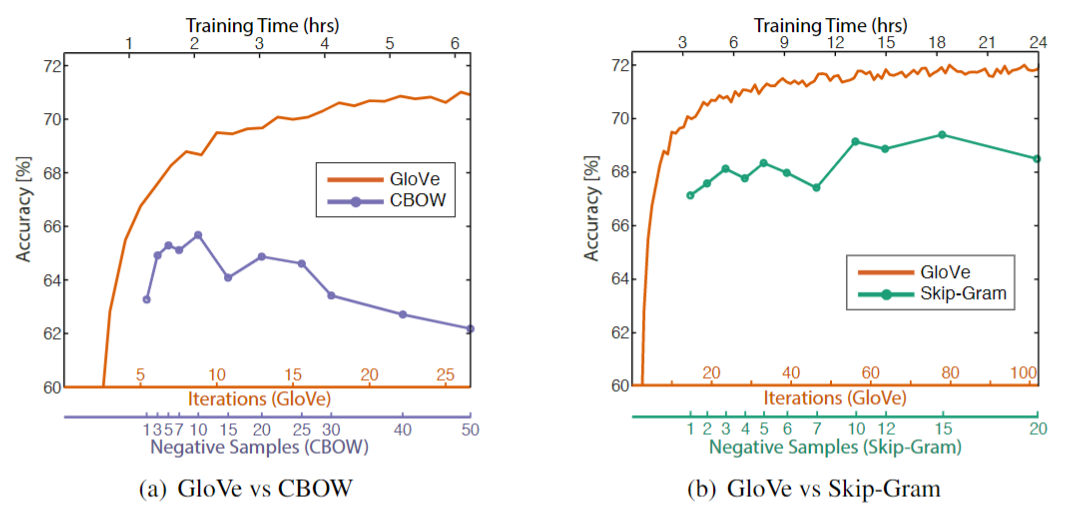
\includegraphics[width=0.8\textwidth]{imgs/table_gloveVSword2vec.png}
\caption{Overall accuracy on word analogy task as a function of training time, which is governed by the number of iterations for GloVe and by the number of negative samples for CBOW (a) and skip-gram (b). Pennington et al. (2014) train 300-dimensional vectors on the same 6B token corpus from Wikipedia and use a symmetric context window of size 10. From \emph{GloVe: Global Vectors for Word Representation}, by Pennington et al., 2014. \url{https://nlp.stanford.edu/pubs/glove.pdf}. Copyright 2014 by Pennington et al.}
\end{figure}
\section{Sequence To Sequence Model} \label{sec:Seq2Seq}

A \textbf{sequence-to-sequence (Seq-to-Seq) model} is often used in natural language processing for machine translation. It takes a sequence of items such as words and outputs another sequence of items. It uses an \textbf{Encoder} that processes the inputs, squashes this information into a \emph{fixed-length} \textbf{context vector}, also known as a \textbf{sentence embedding} or \textbf{thought vector}. The Seq-to-Seq model sends this representation of the source sentence to a \textbf{Decoder} that outputs a target sentence one word at a time, using the context vector (Alammar, 2018a). Commonly, the Encoder and Decoder are \hyperref[sec:RNN]{RNNs} such as \hyperref[sec:LSTM]{LSTMs} or \hyperref[sec:GRU]{GRUs} (described in detail in \nameref{app:Appendix_BasicsRNNLSTM}).


\subsection{Describing Seq-to-Seq Model}

The key feature in the Seq-to-Seq model different from a recurrent neural network (RNN) is the \textbf{context vector}, or the final hidden state of the Encoder. When the Encoder processes the input sequence $\overrightarrow{x} = \{ x_1, ..., x_{T_x} \}$ of individual word vectors $x_t$ in the input sentence $X$, the information is squashed into a \emph{fixed-length} context vector. Formally, a gated recurrent unit (GRU) as the Encoder would output a hidden state given a previous hidden state and the current input: 
$$
h_t = \text{EncoderGRU} \Big( x_t, h_{t-1} \Big)
$$ 
where the context vector named $z$ equals the last hidden state: $z = h_{T_x}$. 
\newline 
The context vector is then passed to the Decoder along with a target token $y_t$ and previous Decoder hidden state $s_{t-1}$ to return a current hidden state, $s_t$:
$$
s_t = \text{DecoderGRU} \Big( y_t, s_{t-1}, z \Big)
$$
The context vector $z$ does not have a time step $t$ subscript, meaning this same context vector from the Encoder is reused each time step in the Decoder. 


\begin{figure}[h]
\vspace{-5pt}
\centering
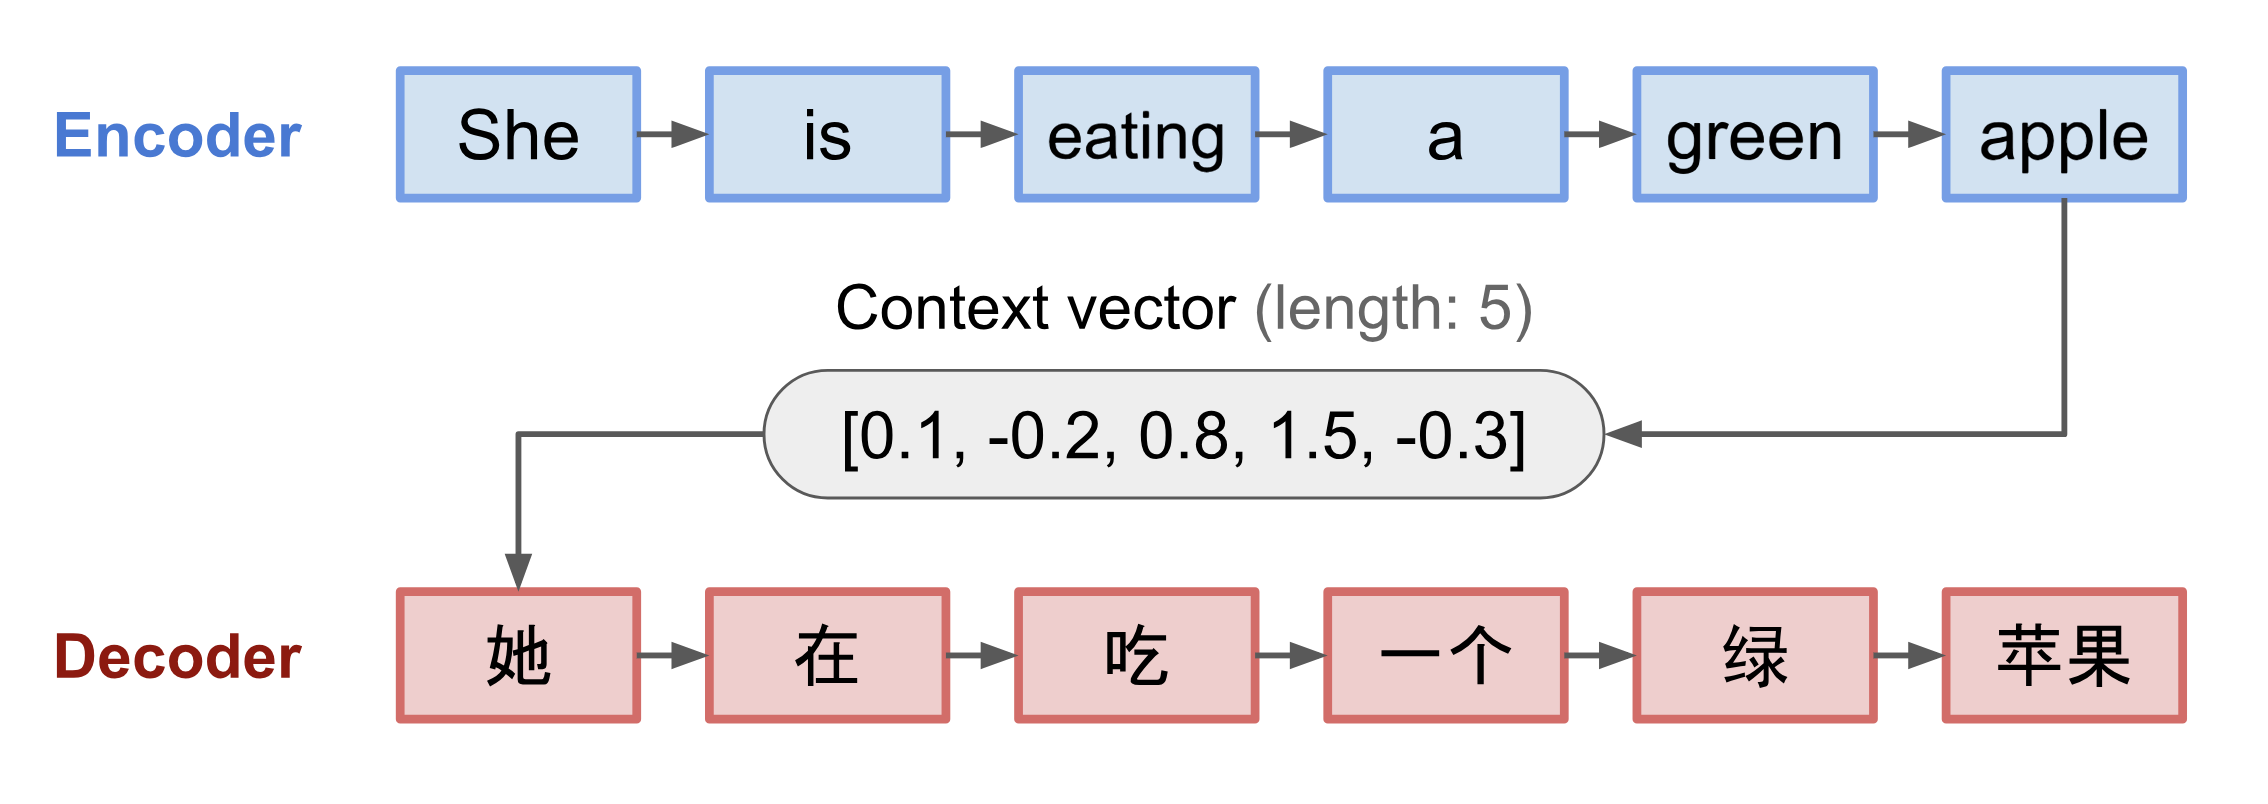
\includegraphics[width=0.6\textwidth]{imgs/seqtoseq_greenapple.png}
\vspace{-5pt}
\caption{\footnotesize Encoder-Decoder with Context Vector in a Seq-to-Seq model, translating the sentence ``She is eating a green apple" to Chinese. From \emph{Attention? Attention!}, by Weng, 2018. \url{https://lilianweng.github.io/lil-log/2018/06/24/attention-attention.html}. Copyright 2018 by Weng.}
\vspace{-5pt}
\end{figure}


\subsection{Problem with Seq-to-Seq Models} \label{sec:ProblemWithSeq2Seq}

However, compressing the inputs into such a \textbf{fixed-length} vector leads to a \textbf{long-term dependency problem} since only the last hidden state of the Encoder is used. Thus, the Seq-to-Seq model becomes incapable of memory, similar to RNNs (see \nameref{app:Appendix_BasicsRNNLSTM}). 

\subsection{The Attention Mechanism} \label{sec:AttentionMechanism}

The \textbf{attention mechanism} was proposed in neural machine translation (NMT) task to memorize longer sentences by ``selectively focusing on parts of the source sentence" as required (Luong et al., 2015). Instead of creating a single context vector $z$ from the Encoder's last hidden state $h_{T_x}$, the attention architecture creates a context vector for each input word or timestep $t$, reducing the information compression problem. This means the attention mechanism uses all the hidden states generated by the Encoder as inputs for the decoding process. For each Decoder output, the attention mechanism ``selectively picks out specific elements from the [input] sequence to produce the [Decoder] output" (Loye, 2019). This essentially creates links between the context vector and entire source input. This is illustrated in a general way in \cref{fig:attention}.

\begin{figure}[h]
\centering
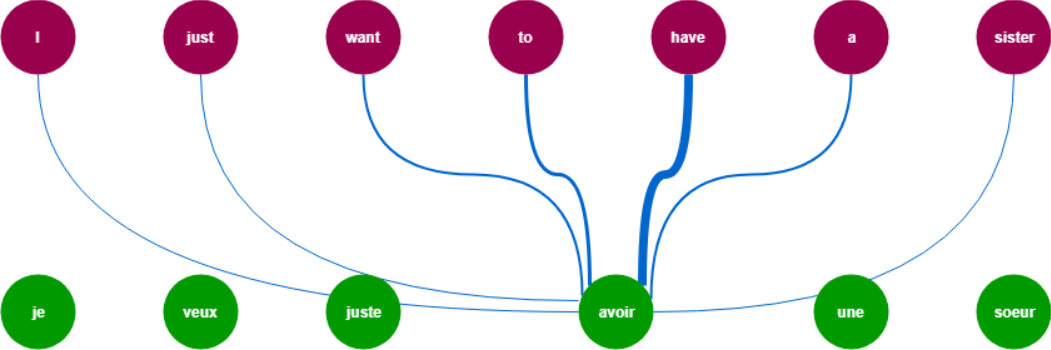
\includegraphics[width=0.6\textwidth]{imgs/attention.png}
\caption{\footnotesize Attention Mechanism: How words are considered for contextual evidence. From \emph{Intuitive Understanding of Seq2seq model and Attention Mechanism in Deep Learning}, by Medium, 2019. \url{https://medium.com/analytics-vidhya/intuitive-understanding-of-seq2seq-model-attention-mechanism-in-deep-learning-1c1c24aace1e}. Copyright n.d by n.d.}
\label{fig:attention}
\end{figure}

\subsection{Seq-to-Seq Model Using Attention}

The key components of a Seq-to-Seq model with attention are its attention forward pass, which computes attention scores, and Decoder forward pass, which outputs the context vector. 

\subsubsection{Forward Pass of Attention}

The attention mechanism is considered a layer in the Seq-to-Seq model with a forward pass that updates parameters. The steps for the forward pass to calculate attention scores $\alpha_{ti}$ is as follows: 
\begin{enumerate}
    \item First, an \textbf{alignment model} $\text{align}$ is used to calculate \textbf{energy scores} $e_{ti}$ that measure how well the ``inputs around position $i$ and the output at position $t$ match" (Bahdanau et al., 2016). The energy scores are weights specifying how much of the Decoder hidden state $s_{t-1}$ and the Encoder hidden state $h_i$ of the source sentence should be considered for each output (Ta-Chun, 2018; Bahdanau et al., 2016). 
    $$
    e_{ti} = \text{align} \Big(s_{t-1}, h_i \Big)
    $$ 
    
    \item Next, the energy score $e_{ti}$ is passed through a feed-forward neural network and softmax to calculate the attention scores, $\alpha_{ti}$:
    $$
    \alpha_{ti} = \frac{\exp{(e_{ti})} } { \sum_{k=1}^{T_x} \exp{(e_{ik})} }
    $$
    Transforming the energy scores via softmax is done to ensure the attention vector $\overrightarrow{\alpha} = \Big \{ \alpha_{ti} \Big \}$ has values normalized between $0$ and $1$. 
\end{enumerate}

%\begin{center}
%    \pythonCodeFile{code/tut3_AttentionClass.py}
%\end{center}

% TODO: line wrapping

\subsubsection{Forward Pass of Decoder}

Once the attention scores have been calculated, the Decoder can calculate the context vector, $c_t$, which is a sum of Encoder hidden states $h_i$ weighted by attention scores $\overrightarrow{\alpha} = \Big \{ \alpha_{ti} \Big \}$ (Ta-Chun, 2018): 
$$
c_t = \sum_{i=1}^{T_x} \alpha_{ti} \cdot h_i
$$

Intuitively, the context vector is an \textbf{expectation}. The attention score $\alpha_{ti}$ is the probability that target word $y_t$ is aligned to (or translated from) an input word $x_j$. Then the $t$-th context vector $c_t$ is the expected hidden state over all hidden states $h_i$ with probabilities $\alpha_{ti}$, where these corresponding energies $e_{ti}$) quantify the importance of Encoder hidden state $h_i$ with respect to the previous Decoder hidden state $s_{t-1}$ in deciding the next Decoder state $s_t$ for generating target word $y_t$. 
\newline Effectively, this is an attention mechanism within the Decoder. By this construction, we can relieve the Encoder of the burden of encoding all source sentence information into a fixed-length vector, so that information can be spread out through the hidden state sequence $\overrightarrow{h} = \Big \{ h_1,...,h_T\Big \}$ and retrieved judiciously by the Decoder (Trevett, 2020). 

%\begin{center}
%    \pythonCodeFile{code/tut3_DecoderClass.py}
%\end{center}


\subsubsection{Forward Pass of Seq-to-Seq Model}

Finally, the Seq-to-Seq model can use the Encoder, Decoder and attention in conjunction. Its forward pass is (Trevett, 2020): 
\begin{enumerate}
    \item Create an output tensor to hold predicted words $\hat{y}$
    
    \item Pass the source sequence $\overrightarrow{x} = \Big \{ x_1, ..., x_T \Big \}$ into the Encoder to receive the contexts $\overrightarrow{z}$ alongside the hidden states $\overrightarrow{h} = \Big \{ h_1, ..., h_T \Big \}$.
    
    \item Set equal the initial Decoder hidden state $s_0$ and last Encoder hidden state $h_T$.
    
    \item Decode within a loop: insert the target token $y_t$ and previous hidden state $s_t$ and all Encoder outputs $\overrightarrow{h}$ into the Decoder to get a prediction $\hat{y}_{t+1}$ and new hidden state $s_t$.
    
    
\end{enumerate}

As an application of the Seq-to-Seq model with attention to the machine translation NLP task, PyTorch code with explanations can be found in \nameref{app:Appendix_Seq2Seq}
%\begin{center}
%    \pythonCodeFile{code/tut3_Seq2Seq.py}
%\end{center}


%\appendix
%\clearpage
%
\section{APPENDIX: Training Neural Networks} \label{app:Appendix_Backprop}

The \textbf{backward propagation of errors} is a method used for training neural network to learn values for the parameters, and is used in conjunction with an optimization method, such as \textbf{gradient descent}. The backward propagation algorithm does a two-phase cycle consisting of error propagation across the graph followed by the parameter weight update.

Neural network training consists of three phases: 1) forward propagation, 2) error calculation, and 3) backward propagation, which itself consists of two phases. To describe this process, we use notation from Gibiansky (2014) and define the following:

\begin{itemize}
    \item $x_i^l$ is the input to the $i$-th in layer $l$, denoted $u_i^l$.
    
    \item $u_i^l$ is the $i$-th \textbf{unit} or \textbf{node} in layer $l$, where $u_i^0$ with $l=0$ means the $i$-th unit in the input layer.
    
    \item $u^L$ is the last (output) layer $L$ of the network.
    
    \item $a_i^l$ is the output \textbf{activation} value of unit $u_i^l$, calculated from a nonlinearity function. 
    
    \item $a^L$ is the \textbf{activation} value in the last layer $L$.
    
\end{itemize}


A \textbf{fully-connected neural network} with $L$ layers has three categories of layers: 

\begin{enumerate}
    \item the \textbf{input } or \textbf{embedding layer} with units $u_i^0$ whose values are determined by the input vectors.
    
    \item the \textbf{hidden layers} with units $u_i^l$ whose values are obtained from previous layers.
    
    \item the \textbf{output layer} with units $u_i^L$ whose values are computed from the last hidden layer.
\end{enumerate} 

The neural network trains to update its weight matrix $W = \Big \{ w_{ij}^l \Big \}$, where $w_{ij}^l$ is the weight value from unit $u_i^l$'s output to another unit $u_j^{l+1}$. Whenever an output is computed from an input, a \textbf{nonlinearity function} $\sigma(\cdot)$ is applied to the input $x$ and this is intuitively seen as ``passing" the input through a layer.


\subsection{Forward Propagation}

\textbf{Forward propagation} or \textbf{forward pass} is the procedure used to propagate an input vector forward through the network layers. The original input is transformed over a series of nonlinear functions to get its activation values $a_i^l$, until the output layer is reached, where the activations are transformed via another nonlinearity to get the final activations $a^L$. 

\subsubsection{Forward Propagation Algorithm}

The \textbf{forward propagation} algorithm is described as follows: 

\begin{enumerate}
    \item Compute the activation values $a_i^l$ for layers with known inputs, using the activation nonlinearity function $\sigma(\cdot)$: 
    $$
    a_i^l = \sigma(x_i^l) + I_i^l
    $$
    
    \item Compute the input values $x_i^l$ for the next layer $l$ from the activations $a_i^l$: 
    $$
    x_i^l = \sum_j w_{ji}^{l-1} a_j^{l-1}
    $$
    
    \item Steps $1$ and $2$ are repeated until the output layer is reached, to get the final output values $a^L$ at the last layer $L$.
\end{enumerate}


\subsection{Error Calculation}

After \textbf{forward propagation}, errors $E(a^L)$ are computed by comparing the network's output with the target predictions, via a loss function, and the error value is calculated for each neuron in the output layer. 

The derivative of the error $E(a^L)$ with respect to computed activations $a_i^L$ is written $\frac {d} {d a_i^L} \Bigg( E(a^L) \Bigg)$ and depends only on the activations. This will be used to optimize the weights to minimize the error in the \textbf{backward propagation algorithm}.
    

\subsection{Backward Propagation}

\textbf{Backward propagation} consists of a first phase when the error values are propagated backwards across the graph, starting from the output layer and moving back over the input layer, until each neuron is updated with the error value. Backpropagation uses these errors to \emph{calculate the gradient of the loss function with respect to the weights in the network}. In the second phase, the gradient of the loss is passed as an argument to the optimization method so that the parameter weights can be adjusted, towards minimizing the loss function. 

\subsubsection{Derivation of Backward Propagation}

In order to use an \textbf{optimization algorithm} to train the network, we must compute the error derivative $\frac {\partial E} {\partial w_{ij}^l} $ with respect to each weight value, $w_{ij}^l$, using the chain rule. 

Also, since $x_i^l = \sum_j w_{ji}^{l-1} a_j^{l-1}$, the partial derivative with respect to any weight is equal to just the activation from the origin neuron: $\frac {\partial x_j^{l+1}} {\partial w_{ij}^l} = a_i^l$, resulting in:

$$
\frac {\partial E} {\partial w_{ij}^l} 
= \frac {\partial E} {\partial x_j^{l+1} } \cdot \frac {\partial x_j^{l+1}} {\partial w_{ij}^l} 
= \frac {\partial E} {\partial x_j^{l+1} } \cdot a_i^l
$$

Now, to decompose further the partial $\frac {\partial E} {\partial x_j^{l+1} }$, we can calculate the partial derivative of the error with respect to the input for the current layer $l$. Using the chain rule and $a_i^l = \sigma(x_i^l) + I_i^l$, we write:
$$
\frac {\partial E} {\partial x_j^l } = \frac {\partial E} {\partial a_j^l } \cdot \frac {\partial a_j^l} {\partial x_j^l }
= \frac {\partial E} {\partial a_j^l } \cdot  \frac {\partial} {\partial x_j^l } \Big( \sigma(x_j^l) + I_j^l \Big)
= \frac {\partial E} {\partial a_j^l }\cdot \sigma '(x_j^l)
$$

Lastly, to decompose the partial $\frac {\partial E} {\partial a_j^l }$, we consider two cases: if we are at the output layer, so $l = L$, or not. When $l = L$, then the partial $\frac {\partial E} {\partial a_j^l }$ is simply the derivative of the error function because the error is just a function of $a_i^L$ and none of the other activations in the output layer: 

$$
\frac {\partial E} {\partial a_j^L } = \frac {\partial} {\partial a_j^L } \Big( E(a^L) \Big)
$$

In the second case, for layers $l$ other than the output layer $L$, we must use the chain rule to sum over all the contributions of the activation in all layers. 
$$
\frac {\partial E} {\partial a_j^l } = \sum \frac {\partial E} {\partial x_j^{l+1} } \cdot \frac {\partial x_j^{l+1}} {\partial a_i^l }
= \sum \frac {\partial E} {\partial x_j^{l+1} } \cdot w_{ij}
$$

This shows that $\frac {\partial E} {\partial a_j^l }$ equals the derivatives of the inputs to the next layer weighted by the importance of the activation $a_i^l$ to each input. Intuitively, this means ``the error at a particular node in layer $l$ is a combination of errors at the next nodes (layer $l+1$), weighted by the size of the contribution of the node in layer $l$ to each of those nodes in layer $l+1$" (Gibiansky, 2014). 

\subsubsection{Backward Propagation Algorithm}

\begin{enumerate}
    \item Calculate the errors at the output layer $L$, with respect to the activations $a_i^L$ at the output layer: 
    $$
    \frac{\partial E}{\partial a_i^L} = \frac{d}{d a_i^L} \Big( E(a^L) \Big)
    $$
    
    \item Calculate the partial derivative of the error with respect to the neuron input $\frac{\partial E}{\partial x_j^l}$ (also denoted ``deltas") at an arbitrary layer $l$:
    $$
    \frac{\partial E}{\partial x_j^l} = \sigma ' (x_j^l) \cdot  \frac{\partial E}{\partial a_j^l}
    $$
    
    \item Calculate errors at the previous layer (this is called backpropagating the errors):
    $$
    \frac{\partial E}{\partial a_i^l} = \sum w_{ij}^l \cdot \frac{\partial E}{\partial x_j^{l+1} }
    $$
    
    \item Repeat Steps $2$ and $3$ until the deltas are known for all layers excluding the input layer. 
    
    \item Complete the steps by calculating the gradient of the error with respect to the weights: 
    $$
    \frac{\partial E}{\partial w_{ij}^l} = a_i^l \cdot \frac{\partial E}{\partial x_j^{l+1}}
    $$
    Intuitively, this means to find derivatives with respect to weights in a given layer, we multiply activations for that layer and deltas for the next layer, so deltas for the input layer never need to be calculated. 
\end{enumerate}
%\clearpage
%\section{Preliminary Building Blocks}

\subsection{Recurrent Neural Networks (RNN)}

\subsubsection{Motivation for RNNs}

Traditional neural networks cannot persist information. As a comparison, while humans do not start thinking from scratch each time they learn something new, neural networks lack memory. Inherently related to sequences, recurrent neural networks use a recurrence or looping mechanism to introduce data persistence in the model to overcome this problem (Colah, 2015). This looping mechanism acts like a ``highway" to flow from one step to the next by passing inputs and modified hidden states along until computing a final prediction (Nguyen, 2018a). 

\begin{figure}[h]
\vspace{-5pt}
\centering
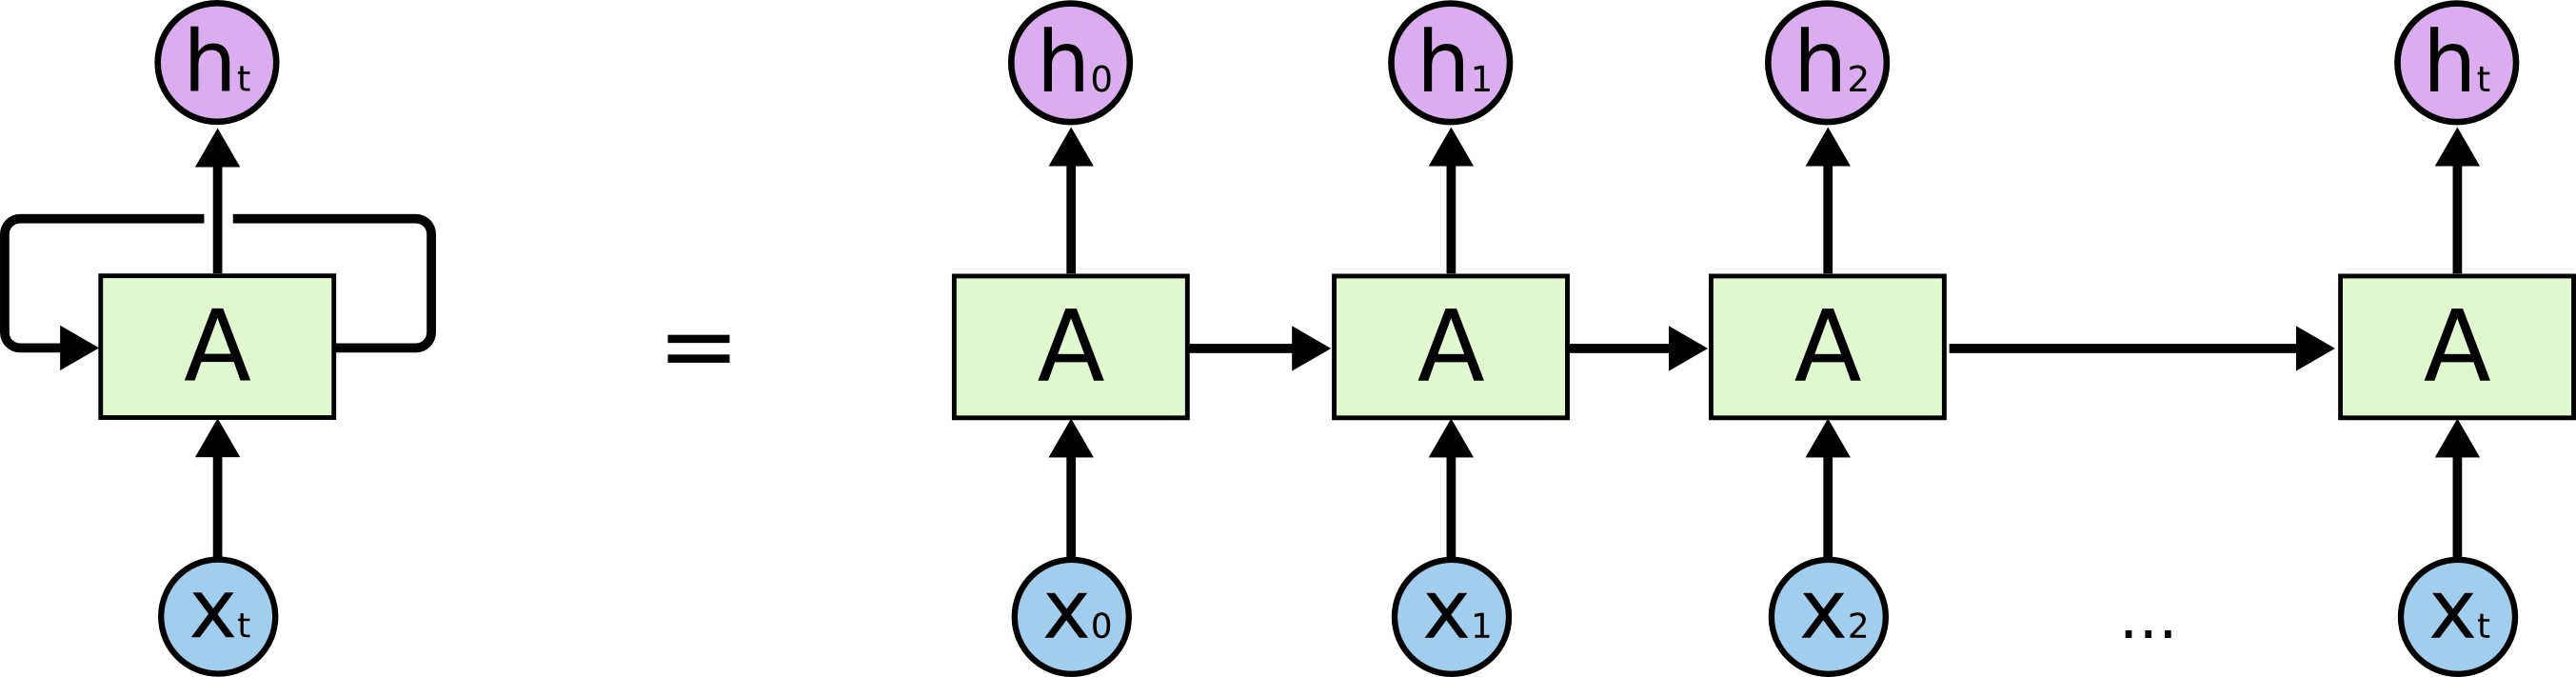
\includegraphics[width=0.6\textwidth]{imgs/rnn_colah_unrolled.png}
\vspace{-5pt}
\caption{\footnotesize Unrolled view of Recurrent Neural Network with Hidden States $h_i$ and inputs $x_i$. From \emph{Understanding LSTMs}, by Colah., 2015. \url{https://colah.github.io/posts/2015-08-Understanding-LSTMs/}. }
\vspace{-5pt}
\end{figure}


\subsubsection{Describing RNNs}

An RNN is a unidirectional language model in that it uses infinite \emph{left} context words to the left of the target word. It is a neural network consisting of a hidden state vector $\overrightarrow{h}$ and output vector $\overrightarrow{y}$ and takes a sequence (sentence) of input symbols (words) $\overrightarrow{x} = \{ x_1, ..., x_T\}$, where each $x_i$ is a word. At each time step $t$ the current hidden state $h_t$ is updated via the formula $h_t = f \Big( h_{t-1}, x_t \Big)$ where $f(\cdot)$ is a nonlinear activation function. The RNN's intermediate task is to predict a probability distribution over an input sequence (sentence) by predicting the next word symbol $x_t$ in the sequence sentence, using left context, so the output at time $t$ is the conditional distribution $P \Big(x_t \; | \; x_{t-1}, ..., x_1 \Big)$. The probability of the entire sequence sentence $\overrightarrow{x}$ is the product of all the probabilities of the individual words, $P(\overrightarrow{x}) = \prod_{t=1}^T P \Big(x_t \; | \; x_{t-1}, ..., x_1 \Big)$ (Cho, 2014). 

Nguyen (2018b) describes the basic workflow of RNNs as follows: 

\begin{enumerate}
    \item First, words are transformed into numeric vectors, allowing the RNN to process the vector sequence, taking one vector at a time. 
    
    \item While processing the inputs in the above step, the RNN passes previous hidden state to the next step of the sequence. The hidden state serves as memory for the network by holding previous information. 
    
    To calculate hidden state for a particular cell in the RNN, the input and previous hidden state are combined to form a vector, which is then passed through a $\text{"tanh"}$ activation function so that its components are squashed betwen $-1$ and $1$ to avoid large values. The output of this operation becomes the new hidden state. 
    
    \item This process is repeated until an output prediction word is generated. 
    
\end{enumerate}


    
\subsection{Long-Short Term Memory Networks (LSTM)}

\subsubsection{Motivation for LSTM: Problem with RNNs}

RNNs suffer from the well known \textbf{long-term dependency problem}. In some prediction tasks, longer context is needed to predict a target word. For instance to predict the last word in the sentence ``I grew up in France ... I speak fluent \emph{French}", a model would need the earlier context word ``France." When this gap between target and context words becomes too large, RNNs cannot learn their relationship, thus showing its lack of handling \textbf{long-term dependencies} (Colah, 2015). 

\begin{figure}[h]
\vspace{-5pt}
\centering
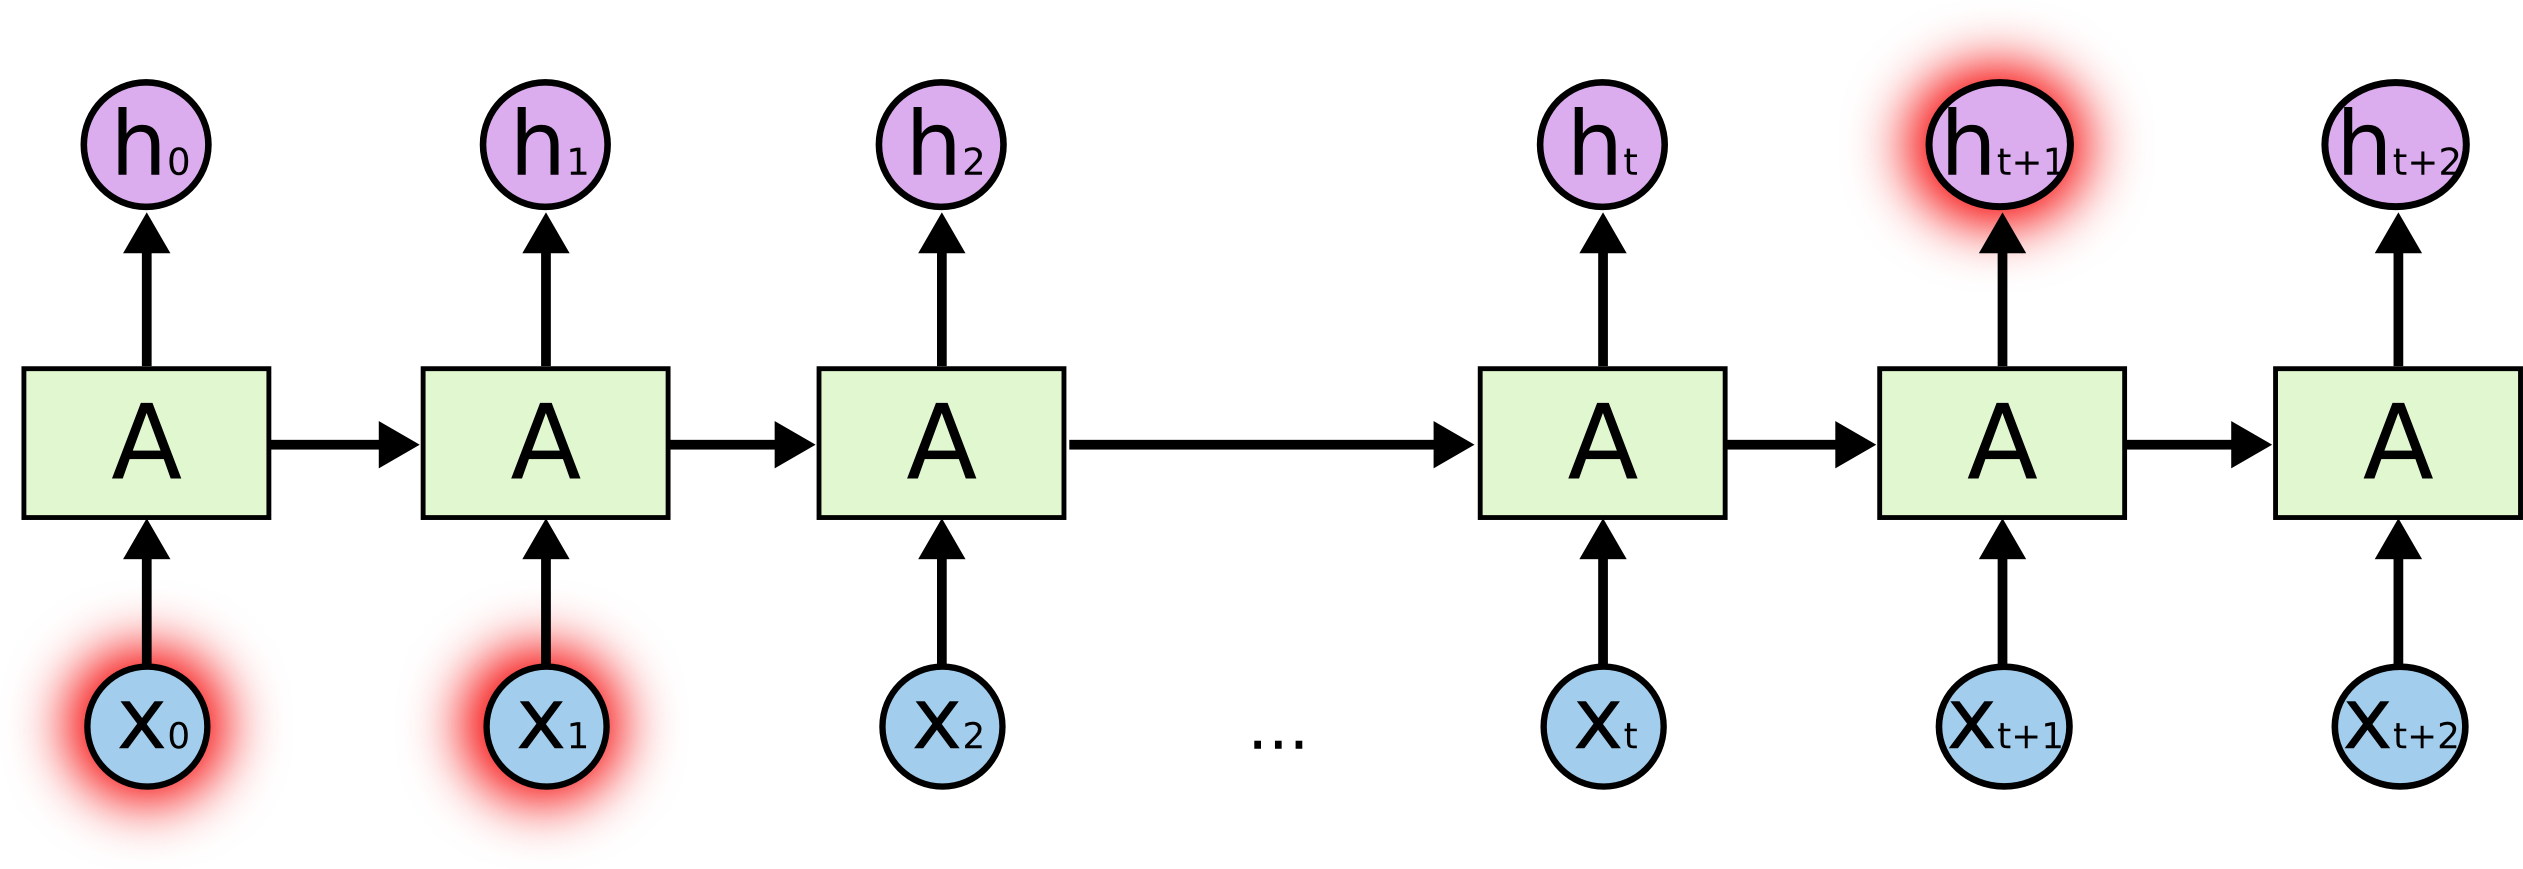
\includegraphics[width=0.6\textwidth]{imgs/rnn_longterm.png}
\vspace{-5pt}
\caption{\footnotesize Long-Term Dependency Problem in RNNs (widening gap between inputs $x_i$ and hidden states $h_j$. From \emph{Understanding LSTMs}, by Colah, 2015. \url{https://colah.github.io/posts/2015-08-Understanding-LSTMs/}. }
\vspace{-5pt}
\end{figure}

The \textbf{short-term memory problem} occurs due to the \textbf{vanishing gradient problem}. During backward propagation of errors through the neural network (described in Appendix A), the gradient shrinks as it back propagates through time and becomes too small to update the parameter weights significantly. This is compounded by the fact that since inputs at any timestep $t$ are dependent on previous $t-1$ outputs, longer sequences require more gradient calculations. Adjustments to earlier layers thus become smaller, causing gradients to shrink exponentially as they are backpropagated through to earlier layers of the RNN. As a result, RNNs ``forget" older history, resulting in short-term memory (Nguyen, 2018b). 


\subsubsection{Describing LSTMs}
A long-short term memory network (LSTM) is a type of RNN that sequentially extracts information from each word in a sentence and embeds the information into a semantic vector. 

Long-short term memory networks (LSTM) learn long-term information by design, contrary to RNNs. LSTMs use features such as \textbf{cell state} and \textbf{gates} to regulate information flow from earlier time steps to later time steps. The gates are separate neural networks that decide which information to add or remove from the cell state, thus explicitly letting the LSTM ``remember" or ``forget" information (Nguyen, 2018b). Simply, LSTMs differ from RNNs in their repeating module since the standard RNN contains a single $\text{tanh}$ activation layer while the LSTM contains the four neural network layers (gates). 

Since LSTMs can accumulate increasingly richer information while parsing the sentence, by the time the last word is reached, the hidden layer of the network provides a \textbf{semantic representation} of the entire sentence (Palangi et al., 2016). 

A core idea in an LSTM is the \textbf{cell state}, which is shown in Figure 11 as the topmost line with the gates merging into it. For example, for a language predicting the next word based on previous ones, the cell state might include the gender of the present subject so that the correct pronouns are used. When a new subject is observed, the cell state should forget the old subject's gender and retain the new one (Colah, 2015). 

From Nguyen (2018b), the gates (neural network layers) regulating information are as follows: 




%%% The forget gate image wrapping ---------------------
\begin{program}
\begin{wrapfigure}{L}{0.45\textwidth}
\vspace{-20pt}
\begin{center}
    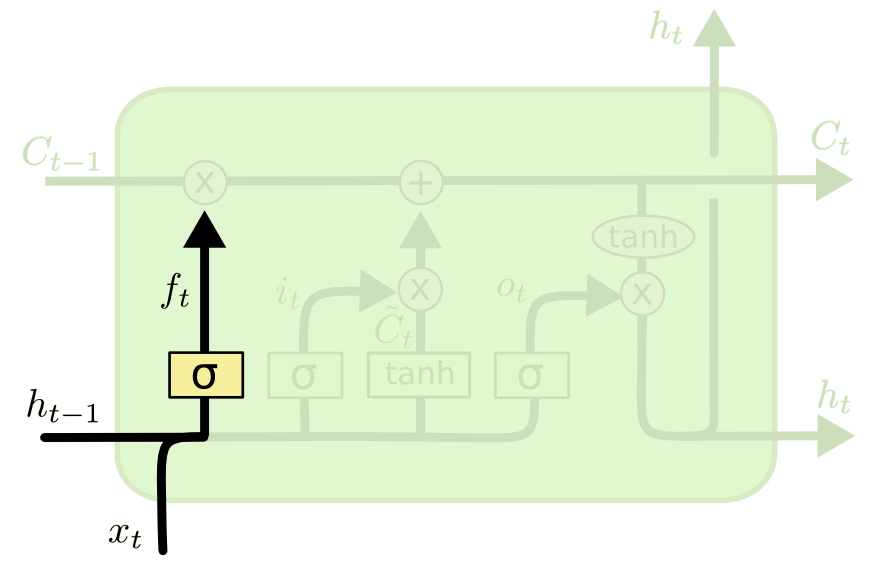
\includegraphics[width=0.4\textwidth]{imgs/lstm_forgetGate.png}
\end{center}
\vspace{-20pt}
\caption{\footnotesize Forget Gate Calculation. From \emph{Understanding LSTMs}, by Colah, 2015. \url{https://colah.github.io/posts/2015-08-Understanding-LSTMs/}. }
\vspace{-5pt}
\end{wrapfigure}

\textbf{Forget Gate: } the forget gate decides information to discard or keep. The previous hidden state $h_{t-1}$ and current input $x_t$ are passed through the sigmoid nonlinearity function. The forget gate outputs a number between $0$ and $1$ for each number in the cell state $C_{t-1}$; values closer to $0$ indicate the forget gate should discard the information and values closer to $1$ should be kept. 
$$
f_t = \sigma \Big( W_f \cdot [h_{t-1}, x_t] + b_f \Big)
$$
where $f_t$ denotes the forget gate for time $t$, $\sigma(\cdot)$ denotes the sigmoid, $W_f$ denotes the weight matrix at the forget layer, and $b_f$ denotes the forget gate's bias term. 
\end{program}


%%% The input gate image wrapping ---------------------
\begin{program}
\begin{wrapfigure}{L}{0.45\textwidth}
\vspace{-20pt}
\begin{center}
    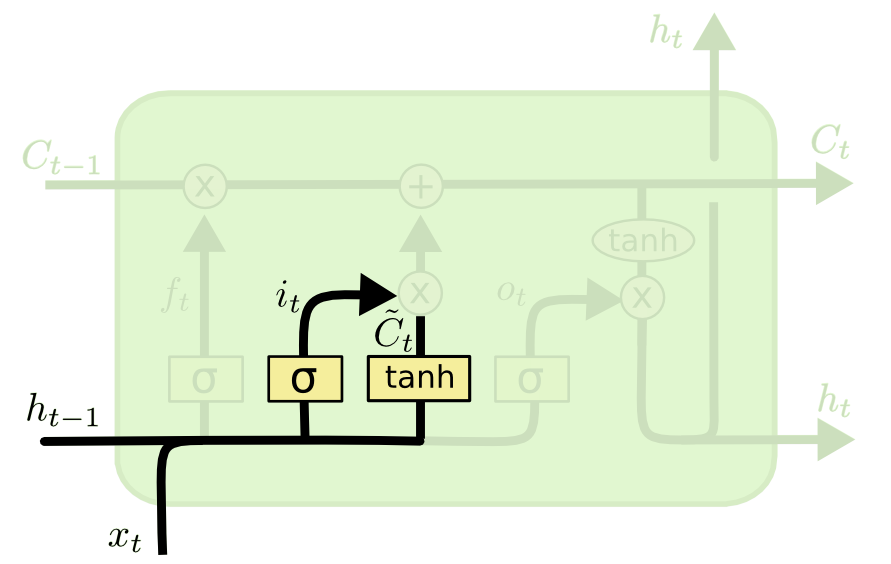
\includegraphics[width=0.4\textwidth]{imgs/lstm_inputGate.png}
\end{center}
\vspace{-20pt}
\caption{\footnotesize Input Gate Calculation. From \emph{Understanding LSTMs}, by Colah, 2015. \url{https://colah.github.io/posts/2015-08-Understanding-LSTMs/}. } 
\vspace{-5pt}
\end{wrapfigure}
\textbf{Input Gate: } the input gate $i_t$ updates the cell state $C_t$. Previous hidden state $h_{t-1}$ and current input $x_t$ are passed though a signmoid function normalize vector cells between $0$ and $1$. The input gate is later used with the cell state to decide how values are updated. 
$$
i_t = \sigma \Big( W_i \cdot [h_{t-1}, x_t] + b_i \Big)
$$
where $i_t$ is the input gate for time $t$, $\sigma(\cdot)$ is the sigmoid, $W_i$ is the weight matrix at the input layer, and $b_i$ is the input gate's bias term. \par \kern 5pt
\end{program}





%%% The cell state gate image wrapping ---------------------
\begin{program}
\begin{wrapfigure}{L}{0.45\textwidth}
\vspace{-20pt}
\begin{center}
    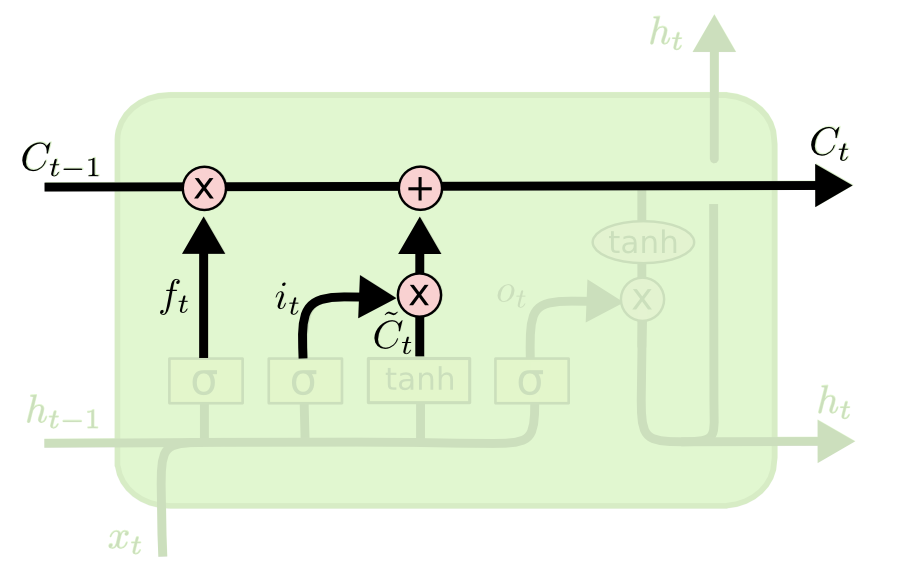
\includegraphics[width=0.4\textwidth]{lstm_cellState.png}    
\end{center}
\vspace{-20pt}
\caption{\footnotesize Cell State Calculation. From \emph{Understanding LSTMs}, by Colah, 2015.\url{https://colah.github.io/posts/2015-08-Understanding-LSTMs/}. }
\vspace{-5pt}
\end{wrapfigure}

\textbf{Cell State: } Current cell state $C_t$ takes $h_{t-1}$ and $x_t$ and normalizes them to be between $-1$ and $1$ via a hyperbolic tangent nonlinearity:
$$
C_t = \tanh \Big( W_C \cdot [h_{t-1}, x_t] + b_C \Big)
$$
where $C_t$ is the cell state for time $t$, $\tanh(\cdot)$ is the hyperbolic tangent, $W_C$ is the weight matrix at the cell state layer, and $b_C$ is the cell state's bias term. 

Next, pointwise multiplications occur to regulate memory in LSTM: 
$$
C_t = f_t \cdot C_{t-1} + i_t \cdot C_t
$$
\end{program}


%%% The output gate image wrapping ---------------------
\clearpage
\begin{program}
\begin{wrapfigure}{L}{0.45\textwidth}
\vspace{-20pt}
\begin{center}
    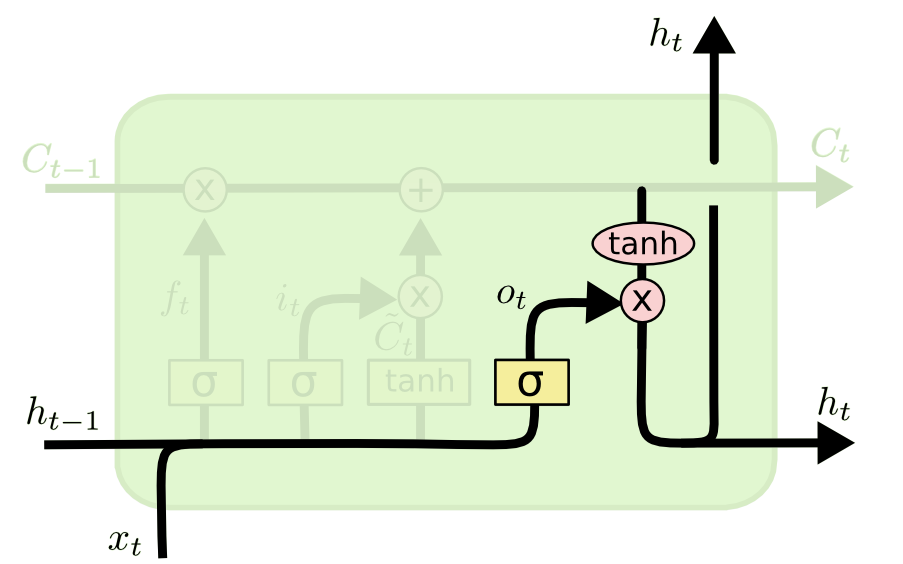
\includegraphics[width=0.4\textwidth]{imgs/lstm_outputGate.png}    
\end{center}
\vspace{-20pt}
\caption{\footnotesize Output Gate Calculation. From \emph{Understanding LSTMs}, by Colah, 2015.\url{https://colah.github.io/posts/2015-08-Understanding-LSTMs/}. }
\vspace{-5pt}
\end{wrapfigure}

\textbf{Output Gate: }the output gate determines the next hidden state by multiplying the previous output state by the cell state that is filtered by the hyperbolic tangent.
$$
\begin{array}{ll}
o_t = \sigma \Big( W_o \cdot [h_{t-1}, x_t] + b_o \Big) \\
h_t = o_t \cdot \tanh(C_t)
\end{array}
$$ 
\newline\newline\newline\newline\newline
\end{program}



\subsection{Gated Recurrent Networks (GRU)}

The gated recurrent unit (GRU) from Cho et al. (2014) is a type of LSTM that ``combines the forget and input gates into a single \textbf{update gate}" and ``merges the cell state and hidden state" (Colah, 2015), resulting with only the reset gate $r_t$ and update gate $z_t$ (Nguyen, 2018b). 

The \textbf{update gate} $z_t$ controls how much information from previous hidden state contributes to current hidden state, acting like a memory cell in the LSTM to remember long-term dependencies (Cho et al., 2014). 

The \textbf{reset gate} $r_t$ signals the hidden state on how to forget previous information. When the reset gate is close to $0$, the initialized hidden state $\Tilde{h}_t$ must ignore previous hidden state $h_{t-1}$ and reset with the current input $x_t$ only. Intuitively, this allows the activation hidden state $h_t$ to forget any irrelevant information for the future (Cho et al., 2014). 

\begin{figure}[h]
\vspace{-5pt}
\centering
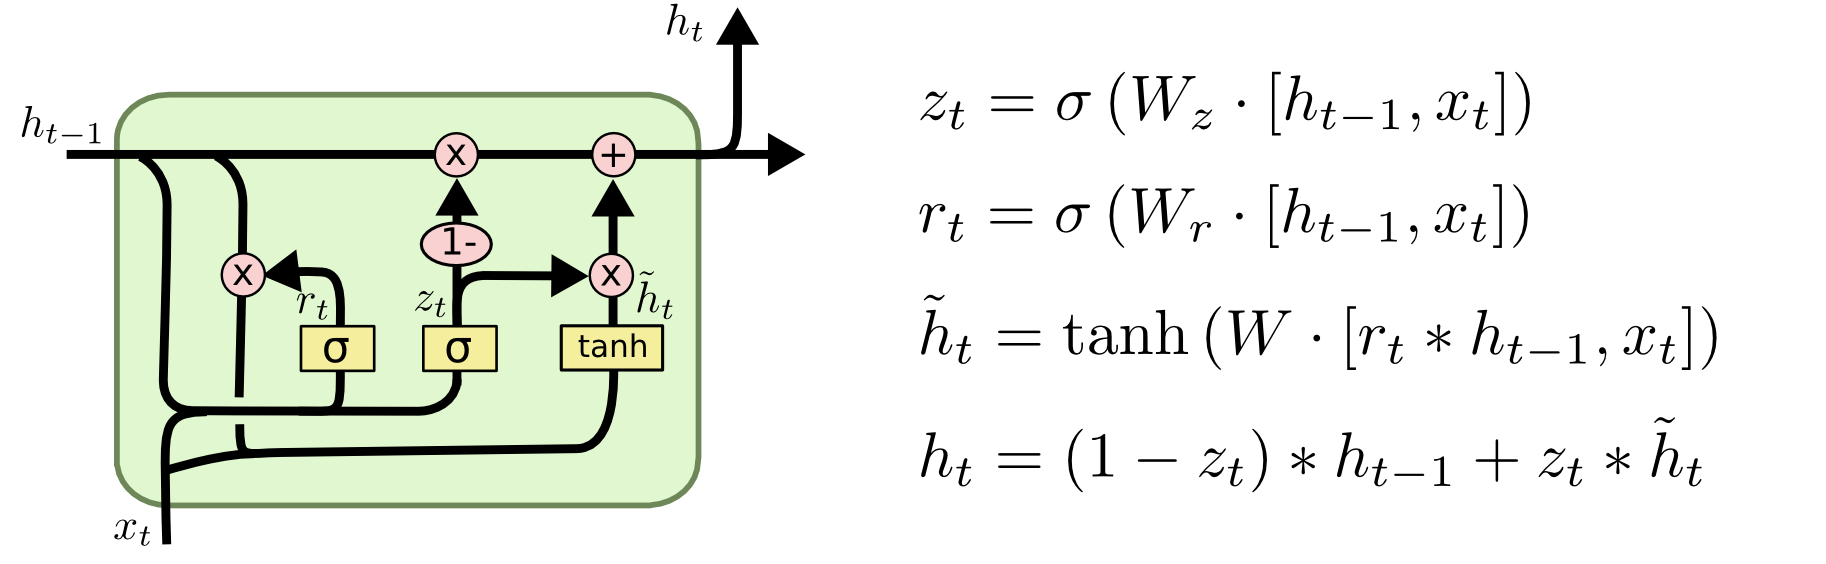
\includegraphics[width=0.8\textwidth]{imgs/gru_withformula.png}
\vspace{-5pt}
\caption{\footnotesize The GRU Cell with Gates. From \emph{Understanding LSTMs}, by Colah, 2015. \url{https://colah.github.io/posts/2015-08-Understanding-LSTMs/}. Copyright 2015 by Colah.}
\vspace{-5pt}
\end{figure}

Nguyen (2018b) notes that since GRU's have fewer tensor operations, they are more efficient than LSTMs during training. 
The GRU adaptively remembers and forgets because each hidden unit has separate reset and update gates so each hidden unit can capture dependencies over different time scales. Frequently active reset gates help the GRU remember short-term dependencies while frequently active update gates help the GRU note long-term dependencies (Cho et al., 2014). 


\subsection{Convolutional Neural Networks (CNN)}
%\clearpage
%\section{APPENDIX: Creating a Skip-Gram Model With PyTorch}

Author: Ana-Maria Vintila, based off work from Srijith Rajamohan based
off the work by Robert Guthrie

Source: https://srijithr.gitlab.io/post/word2vec/

\begin{verbatim}
import os
from IPython.display import Image

pth = os.getcwd()
pth
\end{verbatim}

\begin{verbatim}
'/content/gdrive/My Drive/StatFitScholarshipProject/PythonNeuralNetNLP'
\end{verbatim}

\begin{verbatim}
Image(filename=pth + '/src/NLPstudy/images/Skip-gram.png')
\end{verbatim}

\begin{figure}
\centering
\includegraphics{SkipGram_Rajamohan_files/SkipGram_Rajamohan_3_0.png}
\caption{png}
\end{figure}

Loading the imports:

\begin{verbatim}
import torch
import torch.tensor as Tensor
import torch.nn as nn
import torch.nn.functional as F
import torch.optim as optim
import numpy as np
import urllib.request
from nltk.tokenize import RegexpTokenizer
from nltk.corpus import stopwords
from nltk import word_tokenize
import sklearn
from sklearn.cluster import KMeans
from sklearn.metrics.pairwise import euclidean_distances

torch.manual_seed(1)
\end{verbatim}

\begin{verbatim}
<torch._C.Generator at 0x7f9c3be47370>
\end{verbatim}

\hypertarget{step-1-initialization}{%
\section{Step 1: Initialization}\label{step-1-initialization}}

Here we set the context window size to \(3\) words and the word
embedding dimension to \(10\), and also pass in the text corpora from
which we build vocabulary.

Tokenizing the text occurs later while reading in the data.

\begin{verbatim}
CONTEXT_SIZE = 3
EMBEDDING_DIM = 10

testSentence = """Empathy for the poor may not come easily to people who never experienced it.
They may blame the victims and insist their predicament can be overcome through determination
and hard work.
But they may not realize that extreme poverty can be psychologically and physically
incapacitating — a perpetual cycle of bad diets, health care and education exacerbated
by the shaming and self-fulfilling prophecies that define it in the public imagination.
Gordon Parks — perhaps more than any artist — saw poverty as “the most savage of all human
afflictions” and realized the power of empathy to help us understand it. It was neither an
abstract problem nor political symbol, but something he endured growing up destitute in rural
Kansas and having spent years documenting poverty throughout the world, including the United
States.
That sensitivity informed “Freedom’s Fearful Foe: Poverty,” his celebrated photo essay published
 in Life magazine in June 1961. He took readers into the lives of a Brazilian boy, Flavio
 da Silva, and his family, who lived in the ramshackle Catacumba favela in the hills outside
 Rio de Janeiro. These stark photographs are the subject of a new book, “Gordon Parks: The
  Flavio Story” (Steidl/The Gordon Parks Foundation), which accompanies a traveling exhibition
  co-organized by the Ryerson Image Centre in Toronto, where it opens this week, and
  the J. Paul Getty Museum. Edited with texts by the exhibition’s co-curators, Paul Roth and
  Amanda Maddox, the book also includes a recent interview with Mr. da Silva and essays by
  Beatriz Jaguaribe, Maria Alice Rezende de Carvalho and Sérgio Burgi.
""".split()
\end{verbatim}

\hypertarget{step-2-build-the-n-grams}{%
\section{\texorpdfstring{Step 2: Build the
\(n\)-grams}{Step 2: Build the n-grams}}\label{step-2-build-the-n-grams}}

Next we build the \(n\)-grams, or sequence of words, as a list of
tuples.

Each tuple is ({[} \texttt{word}\(_{i-2}\), \texttt{word}\(_{i-1}\) {]},
\texttt{targetWord})

\begin{verbatim}
ngrams = []
for i in range(len(testSentence) - CONTEXT_SIZE):
    tup = [testSentence[j] for j in np.arange(i + 1, i + CONTEXT_SIZE + 1)]
    # skip-gram way of appending:
    ngrams.append( (testSentence[i], tup) )
    # cbow# ngrams.append( (tup, testSentence[i + CONTEXT_SIZE]) )
\end{verbatim}

\begin{verbatim}
ngrams[:20] # showing a few sample n-grams
\end{verbatim}

\begin{verbatim}
[('Empathy', ['for', 'the', 'poor']),
 ('for', ['the', 'poor', 'may']),
 ('the', ['poor', 'may', 'not']),
 ('poor', ['may', 'not', 'come']),
 ('may', ['not', 'come', 'easily']),
 ('not', ['come', 'easily', 'to']),
 ('come', ['easily', 'to', 'people']),
 ('easily', ['to', 'people', 'who']),
 ('to', ['people', 'who', 'never']),
 ('people', ['who', 'never', 'experienced']),
 ('who', ['never', 'experienced', 'it.']),
 ('never', ['experienced', 'it.', 'They']),
 ('experienced', ['it.', 'They', 'may']),
 ('it.', ['They', 'may', 'blame']),
 ('They', ['may', 'blame', 'the']),
 ('may', ['blame', 'the', 'victims']),
 ('blame', ['the', 'victims', 'and']),
 ('the', ['victims', 'and', 'insist']),
 ('victims', ['and', 'insist', 'their']),
 ('and', ['insist', 'their', 'predicament'])]
\end{verbatim}

\hypertarget{step-3-create-vocabulary}{%
\section{Step 3: Create Vocabulary}\label{step-3-create-vocabulary}}

Create the vocabulary by converting the text into a \texttt{set} to
remove duplicate words.

\begin{verbatim}
vocabulary = set(testSentence)
\end{verbatim}

\begin{verbatim}
len(vocabulary)
list(vocabulary)[:20] # showing first 20 words in vocabulary
\end{verbatim}

\begin{verbatim}
['lived',
 'psychologically',
 'prophecies',
 'Gordon',
 'Silva',
 'They',
 'abstract',
 'perpetual',
 'hills',
 'Silva,',
 'power',
 'magazine',
 'imagination.',
 'something',
 'recent',
 'all',
 'may',
 'understand',
 'cycle',
 'who']
\end{verbatim}

\hypertarget{step-4-create-map-of-words-to-indices}{%
\section{Step 4: Create Map of Words to
Indices}\label{step-4-create-map-of-words-to-indices}}

Creating word to index map that prints the key (word) corresponding to
the given index in the dictionary argument. Basically, we get a list of
tuples (number, word) from zipping the sequence \(0,1,2,3 ....\) with
the vocabulary word list.

\begin{verbatim}
wordToIndex = {word : i for i, word in enumerate(vocabulary)}
\end{verbatim}

\begin{verbatim}
# Showing first 20 word to index pairs
len(wordToIndex)
itemsList = list(wordToIndex.items())
itemsList[:20]
\end{verbatim}

\begin{verbatim}
[('lived', 0),
 ('psychologically', 1),
 ('prophecies', 2),
 ('Gordon', 3),
 ('Silva', 4),
 ('They', 5),
 ('abstract', 6),
 ('perpetual', 7),
 ('hills', 8),
 ('Silva,', 9),
 ('power', 10),
 ('magazine', 11),
 ('imagination.', 12),
 ('something', 13),
 ('recent', 14),
 ('all', 15),
 ('may', 16),
 ('understand', 17),
 ('cycle', 18),
 ('who', 19)]
\end{verbatim}

\begin{verbatim}
def printKey(iWord, wordToIndexDict):
    """
    Prints the key (the word) corresponding to the given index in the given dictionary.

    :param iWord: index of a word in the given dict
    :param wordToIndexDict: the dictionary
    :return: key
    """
    for key, index in wordToIndexDict.items():
        if(index == iWord):
            print(key)



def clusterEmbeddings(filename, numClusters):
    X = np.load(filename)
    kmeans = KMeans(n_clusters=numClusters, random_state=  0).fit(X) # from sklearn
    center = kmeans.cluster_centers_
    distances = euclidean_distances(X, center)

    for i in np.arange(0, distances.shape[1]):

        # get the index of the minimum distance in the ith row of the dist matrix
        iMinWord = np.argmin(distances[:, i])
        print(iMinWord)
        printKey(iWord=iMinWord, wordToIndexDict= wordToIndex)


def readData(filePath):
    tokenizer = RegexpTokenizer(r'\w+')
    data = urllib.request.urlopen(filePath)
    data = data.read().decode('utf8')
    tokenizedData = word_tokenize(data)

    # note: stopwords are from nltk
    stopWordsSet = set(stopwords.words('english'))
    stopWordsSet.update(['.',',',':',';','(',')','#','--','...','"'])
    cleanedWords = [word for word in tokenizedData if word not in stopWordsSet]

    return cleanedWords
\end{verbatim}

\hypertarget{step-6-create-skip-gram-model}{%
\section{Step 6: Create Skip-Gram
Model}\label{step-6-create-skip-gram-model}}

The skip-gram neural network has three components:

\begin{enumerate}
\def\labelenumi{\arabic{enumi}.}
\tightlist
\item
  embedding layer, created using pytorch's \texttt{nn.Embedding}, to
  convert tensors into word embeddings.
\item
  hidden layer, in this case it is a linear layer.
\item
  output layer, in this case also linear layer.
\end{enumerate}

\hypertarget{forward-pass-of-skip-gram}{%
\subsubsection{Forward Pass of
Skip-Gram:}\label{forward-pass-of-skip-gram}}

\begin{enumerate}
\def\labelenumi{\arabic{enumi}.}
\tightlist
\item
  Convert the tensor \texttt{inputs} to word embeddings via the
  skip-gram's \texttt{nn.Embedding} layer
\item
  Pass the embeddings to the hidden layer and transform the result using
  the \texttt{relu} function
\item
  Transform the hidden layer results using the output layer.
\item
  Finally, create a probability distribution over words using the
  \texttt{softmax} function. (Here we actually use the
  \texttt{log\_softmax} so the results are log probabilities instead of
  probabilities. )
\end{enumerate}

\hypertarget{predictions}{%
\subsubsection{Predictions:}\label{predictions}}

To generate predictions we need to execute the \texttt{forward} pass of
the skip-gram model and get the index of the maximum probability from
the output layer. Then that index is used to find the corresponding
prediction word.

\begin{verbatim}
class SkipGramModeler(nn.Module):

    def __init__(self, vocabSize: int, embeddingDim: int, contextSize: int):
        super(SkipGramModeler, self).__init__()

        # see docs: https://hyp.is/cv2pSAeqEeqIRHv7JAjgtA/pytorch.org/docs/stable/nn.html
        # num_embeddings = size of the dictionary embeddings
        # embedding_dim = the size of each embedding vector
        # Creating an embedding model that contains (vocabSize) tensors each of size (embeddingDim)
        self.embeddings = nn.Embedding(num_embeddings=vocabSize,
                                       embedding_dim=embeddingDim,
                                       padding_idx=contextSize)

        # see nn.Linear docs
        # https://hyp.is/XEDPhgerEeqFhHssJYoa-w/pytorch.org/docs/stable/nn.html
        # note: in_features = size of each input sample
        # note: out_features = size of each output sample
        self.hiddenLayer = nn.Linear(in_features=embeddingDim,
                                     out_features=128)

        self.outputLayer = nn.Linear(in_features=128,
                                     out_features=contextSize * vocabSize)


    def forward(self, inputs: Tensor) -> Tensor:
        """

        :param inputs: 1-dim tensor
        :return:
        """
        # note: -1 implies the size inferred for that index from the size of data
        # is a tensor
        inputEmbeddings: Tensor = self.embeddings(inputs).view((1,-1))

        # output at hidden layer
        hiddenRELUResults: Tensor = F.relu(self.hiddenLayer(inputEmbeddings))
        # output at final layer
        outputResults: Tensor = self.outputLayer(hiddenRELUResults)

        logProbs: Tensor = F.log_softmax(input=outputResults, dim=1).view(CONTEXT_SIZE, -1)

        return logProbs



    def predict(self, inputStr: str, wordToIndexDict: dict) -> list:
        """

        :param inputStr: single word (targetword) from which we predict context list
        :return:
        """
        contextIndices: Tensor = torch.tensor([wordToIndexDict[inputStr]],
                                              dtype=torch.long)

        logProbs: Tensor = self.forward(contextIndices)

        # get index of maximum log probability from output layer
        #iMaxLogProbs: Tensor = torch.argmax(logProbs)

        # returns log probs sorted in descending order and
        # iSorted = indices of elements in the input tensor
        logProbsDecr, iSorted = logProbs.sort(descending=True)

        # same as logs.squeeze()[:3] (erasing first dimension)
        # since the tensor is [[...]]

        # getting sorted indices, the first one in each row of iSorted
        # (there are three rows in the iSorted, 2-dim tensor)
        numRows, numCols = iSorted.size()
        iFirstCol = 0
        indices = [iSorted[r][iFirstCol] for r in np.arange(0, numRows)]


        keyIndFilteredPairs: list = []

        for i in indices:

            keyIndFilteredPairs.append( [ (key, index)
                                       for key, index in wordToIndexDict.items()
                                       if index == i ]  )

        return keyIndFilteredPairs

    def printLayerParamers(self):
        for name, child in self.named_children():
            print("\nname = {}, child = {}".format(name, child))

            # TODO: type of child?
            for names, params in child.named_parameters():
                print("names = {}, params = {}".format(names, params))
                print("params.size() = {}".format(params.size()))


    def writeEmbeddingToFile(self, filename: str):
        for i in self.embeddings.parameters():
            weights = i.data.numpy()
        np.save(filename, weights)
\end{verbatim}

\begin{verbatim}
# Trial : testing out the predict() inner workings

inputStr = "psychologically"

contextIndices: Tensor = torch.tensor([wordToIndex[inputStr]],
                                      dtype=torch.long)
print("contextIndices: ", contextIndices)
print("contextIndices dim: ", contextIndices.dim())
print("contextIndices size: ", contextIndices.size())

\end{verbatim}

\begin{verbatim}
contextIndices:  tensor([137])
contextIndices dim:  1
contextIndices size:  torch.Size([1])
\end{verbatim}

\begin{verbatim}
dummyModel = SkipGramModeler(vocabSize=len(vocabulary), embeddingDim=EMBEDDING_DIM,
                         contextSize=CONTEXT_SIZE)

logProbs: Tensor = dummyModel(contextIndices)


# returns log probs sorted in descending order and
# iSorted = indices of elements in the input tensor
logProbsDecr, iSorted = logProbs.sort(descending=True)
print("logProbsDecr dim : ", logProbsDecr.dim())
print("logProbsDecr shape : ", logProbsDecr.shape)
print("logProbsDecr squeezed: ", logProbsDecr.squeeze()[:, :5])
print("logProbsDecr squeezed dim :  ", logProbsDecr.squeeze().dim())
print("logProbsDecr squeezed shape: ", logProbsDecr.squeeze().shape)

print("\niSorted dim: ", iSorted.dim())
# note: in this case, squeezing is same as the original tensor; has no effect
print("iSorted: ", iSorted[:, :5])

logProbsDecr = logProbsDecr.squeeze()   # logProbsDecr[0][:3]
iSorted = iSorted.squeeze()



# getting sorted indices, the first one in each row of iSorted
# (there are three rows in the iSorted, 2-dim tensor)
numRows, numCols = iSorted.size()
iFirstCol = 0
indices = [iSorted[r][iFirstCol] for r in np.arange(0, numRows)]

print("\nindices = ", indices)


# it length will be numRows of iSorted (numRows = 3)
# which equals CONTEXT_SIZE
keyIndFilteredPairs: list = []

for i in indices:

    keyIndFilteredPairs.append( [ (key, index)
                                  for key, index in wordToIndex.items()
                                  if index == i ]  )

print("\nlength of key,ind pairs: ", len(keyIndFilteredPairs))
print("keyIndFilteredPairs: ", keyIndFilteredPairs)
\end{verbatim}

\begin{verbatim}
logProbsDecr dim :  2
logProbsDecr shape :  torch.Size([3, 195])
logProbsDecr squeezed:  tensor([[-5.7581, -5.7919, -5.8080, -5.8146, -5.8202],
        [-5.5920, -5.6021, -5.6844, -5.7157, -5.7189],
        [-5.6294, -5.6362, -5.6638, -5.6691, -5.7091]],
       grad_fn=<SliceBackward>)
logProbsDecr squeezed dim :   2
logProbsDecr squeezed shape:  torch.Size([3, 195])

iSorted dim:  2
iSorted:  tensor([[107,  95,  74,  63,  11],
        [142, 106, 100,  10,  93],
        [167,   1,  44,   9,   8]])

indices =  [tensor(107), tensor(142), tensor(167)]

length of key,ind pairs:  3
keyIndFilteredPairs:  [[('traveling', 107)], [('outside', 142)], [('Foundation),', 167)]]
\end{verbatim}

\hypertarget{step-7-train-the-skip-gram-model}{%
\section{Step 7: Train the Skip-Gram
Model}\label{step-7-train-the-skip-gram-model}}

Training the model requires the following steps:

\begin{enumerate}
\def\labelenumi{\arabic{enumi}.}
\tightlist
\item
  Convert the context words into integer indices using the
  \texttt{wordToIndex} dictionary, and make their type a
  \texttt{Tensor}.
\item
  Set the model gradients to zero so they do not accumulate artificially
  (feature of pytorch)
\item
  Do the \texttt{forward} pass of the Skip-Gram model, resulting in the
  log probabilities of the context words.
\item
  For each word in the correct target context wrods, convert it to an
  index using the \texttt{wordToIndex} dictionary and wrap it in a
  \texttt{Tensor} type.
\item
  Compute the loss between the log probabilities and target contexts.
\item
  Do the \texttt{backward} pass over the neural network to update the
  gradients by calling \texttt{loss.backward()}.
\item
  Do one step using the optimizer, so that weights are updated using
  stochastic gradient descent.
\item
  Increment the total loss by this epoch's current loss.
\end{enumerate}

\begin{verbatim}
%time

learningRate = 0.001
NUM_EPOCHS = 550

losses = []
lossFunction = nn.NLLLoss()
skipGramModel = SkipGramModeler(vocabSize = len(vocabulary),
                        embeddingDim=EMBEDDING_DIM,
                        contextSize=CONTEXT_SIZE)
# Using the stochastic-gradient descent optimizer.
optimizer = optim.SGD(skipGramModel.parameters(), lr = learningRate)

# Preserve the data by freezing the embedding layer
#skipGramModel.freezeLayer("embeddingsSkipGram")

for epoch in range(NUM_EPOCHS):
    totalLoss = 0

    # note: skipgram predicts CONTEXT from single word
    # while CBOW predicts single TARGET word from CONTEXT list
    for contextWord, targetContext in ngrams:

        # Step 1: Prepare the inputs to be passed to the model (means
        # turn the words into integer indices and wrap them in tensors)
        contextIndices: Tensor = torch.tensor([wordToIndex[contextWord]],
                                              dtype=torch.long)

        # Step 2:
        skipGramModel.zero_grad()

        # Step 3: run forward pass, getting log probs over the next words
        logProbs = skipGramModel(contextIndices)

        # Step 4: compute loss, where target word is wrapped in a tensor
        targetContextTensor: Tensor = torch.tensor([wordToIndex[w] for w in targetContext],
                                           dtype=torch.long)

        loss = lossFunction(logProbs, targetContextTensor)

        # Step 5: do backward pass and update gradient
        loss.backward()
        optimizer.step()

        totalLoss += loss.item()

    if(epoch % 50 == 0):
        print("Epoch = {}, Total loss = {}".format(epoch, totalLoss))

    losses.append(totalLoss)
\end{verbatim}

\begin{verbatim}
CPU times: user 2 µs, sys: 0 ns, total: 2 µs
Wall time: 4.53 µs
Epoch = 0, Total loss = 1640.9999227523804
Epoch = 50, Total loss = 1518.4927296638489
Epoch = 100, Total loss = 1414.1443753242493
Epoch = 150, Total loss = 1292.492782831192
Epoch = 200, Total loss = 1149.2484674453735
Epoch = 250, Total loss = 998.4024060964584
Epoch = 300, Total loss = 857.8129457235336
Epoch = 350, Total loss = 742.0071568489075
Epoch = 400, Total loss = 655.678228020668
Epoch = 450, Total loss = 594.8056415319443
Epoch = 500, Total loss = 552.3266983032227
\end{verbatim}

\begin{verbatim}
skipGramModel.predict(inputStr = "psychologically", wordToIndexDict=wordToIndex)
skipGramModel.writeEmbeddingToFile(filename = pth + "/src/NLPstudy/SkipGramModel/rajamohan_skipgram_embeddings.txt")
\end{verbatim}

\begin{verbatim}
clusterEmbeddings(filename = pth + "/src/NLPstudy/SkipGramModel/rajamohan_skipgram_embeddings.txt.npy", numClusters=5)
\end{verbatim}

\begin{verbatim}
3
shaming
28
victims
191
It
18
book,
87
Silva,
\end{verbatim}

\begin{verbatim}
\end{verbatim}

%\clearpage
%\input{Appendix_Tutorial_CBOWModel.tex}
%\clearpage
%\section{PyTorch Tutorial: Seq-To-Seq Model With Attention}


%\clearpage
%\input{Appendix_Tutorial_TransformerModel.tex}
%\clearpage
%\input{Appendix_Tutorial_LSTMFromScratch.tex}
% ----------------------------------------------------------------
% Report End

\end{document}